\documentclass[a4paper]{article}
\usepackage[portuguese]{babel}
\usepackage[utf8]{inputenc}
\usepackage{amsmath}
\usepackage{graphicx}
\usepackage[margin=2cm]{geometry}
\setlength{\parindent}{0cm}
\usepackage{setspace}
\usepackage[colorinlistoftodos]{todonotes}
\usepackage{subfig}
\usepackage{pdfpages}
\usepackage{placeins}
\usepackage{indentfirst}
\usepackage{float}

\begin{document}
\onehalfspace
% Capa
\begin{titlepage}
    \begin{center}
       {\Large UNIVERSIDADE FEDERAL DO PARANÁ}\\[3cm]
       {\Large BRUNA RIBEIRO RESENDE\\[0.5cm]WENDEURICK SILVERIO}\\[8cm]
        {\Large PROJETO DE CONVERSORES CC-CC} \\[0.5cm]
        {\Large CONVERSOR ELEVADOR DE TENSÃO (BOOST)} \\[8cm]
      %  {\Large CONTROLE DE INCLINAÇÃO DE PLATAFORMA \\[0.5cm]COM SENSOR DE ULTRASSOM}\\[6cm]
        {\Large CURITIBA\\[0.5cm]2018}
        \vfill
    \end{center}
\end{titlepage}

\begin{titlepage}
    \begin{center}
       
       {\Large BRUNA RIBEIRO RESENDE\\[0.5cm]WENDEURICK SILVERIO}\\[6cm]
        {\Large PROJETO DE CONVERSORES CC-CC} \\[0.5cm]
        
      {\Large CONVERSOR ELEVADOR DE TENSÃO (BOOST)}\\[1cm]
      \end{center}

  \hspace{.6\textwidth} %posiciona a minipage
   \begin{minipage}{.45\textwidth}
   \large Relatório apresentado à disciplina de Conversores CC-CC e Inversores do curso de Engenharia Elétrica do Departamento de Engenharia Elétrica, Setor de Tecnologia da Universidade Federal do Paraná.\\[0.5cm]
Orientador: Prof. Dr. João Américo Vilela Júnior.\\[6cm]
  \end{minipage}
  \vfill

      \begin{center}
      {\Large CURITIBA\\[0.5cm]2018}
        \vfill
      \end{center}
            
    
\end{titlepage}

{\Large
% inserir o sumario
\tableofcontents
\cleardoublepage

%Textos do trabalho
\Large
\section{Introdução}

Por fim, são apresentadas e discutidas as conclusões e observações de cada etapa do desenvolvimento do projeto proposto.

\section{Objetivos}

\subsection{Objetivo Geral}
\Large
A finalidade do projeto apresentado se resume na implementação de uma das topologias de conversor CC-CC, neste caso, o conversor elevador de tensão (\textit{Boost}). Esta implementação seguirá as seguintes especificações:

\begin{table}[H] \large
\centering
\caption{Especificações do Conversor CC-CC Boost}
\label{tab1}
\begin{tabular}{lc}
\multicolumn{2}{c}{\textbf{Parâmetros de Implementação}}     \\
\hline
Tensão de Entrada       & $9-18V_{cc}$ \\
Tensão de Saída         & $24V_{cc}$   \\
Frequência de Comutação & $250kHz$        \\
Potência do Conversor   & $30W$ \\ \hline
\end{tabular}
\end{table}

\subsection{Objetivos Específicos}

\begin{itemize}
\item Especificação dos componentes do conversor;
\item Projeto do indutor;
\item Definição e simulação do compensador;
\item Layout e confecção da placa de circuito impresso;
%\item Simulação do conversor;
\item Testes em bancada para verificação do funcionamento do conversor \textit{Boost} de acordo com as especificações do projeto.
\end{itemize}

\section{Especificação de Componentes do Conversor}
Nesta seção é realizado o levantamento dos dados necessários para a determinação dos componentes de um conversor CC-CC elevador (\emph{Boost}) (Figura \ref{fig:sch}), cuja a especificação é dada a seguir: $V_{in} = 9-18V$,
$V_{out} = 24V$, $P = 30W$ e $Freq = 250k Hz$.
\FloatBarrier
\begin{figure}[H]
	\centering
	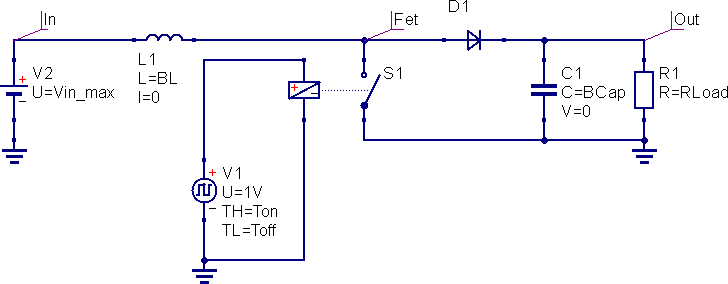
\includegraphics[width=0.85\textwidth]{sch.png}
	\caption{Esquemático do conversor Boost.}
	\label{fig:sch}
\end{figure}
\FloatBarrier
A partir desses parâmetros, tem-se os valores da carga e sua corrente média:

\begin{equation}
\label{eq:r_out}
\begin{split}
R_{out} & = \frac{V_{out}^{2}}{P} \\
& = \frac{{24}^{2}}{30} = 19,2 \Omega
\end{split}
\end{equation}

\begin{equation}
\label{eq:i_out_med}
\begin{split}
I_{{out}_{med}} & = \frac{P}{V_{out}} \\
& = \frac{30}{24} = 1,250 A
\end{split}
\end{equation}

Com isso, através do \textit{software} Qucs, simulou-se o circuito da Figura \ref{fig:sch}, obtendo-se os parâmetros a seguir.

%\pagebreak

\begin{enumerate}
% ---------------------------------------------
\item Capacitor
\begin{enumerate}
\item Capacitância \\
A escolha da capacitância leva em conta a variação da tensão de saída (${\triangle}_{V_{out}}$) e a razão cíclica (\emph{D}) da chave. \\
O ciclo de trabalho foi calculado para o pior caso, ou seja, quando \emph{D} assume seu valor máximo (quando a tensão de entrada assume o valor mínimo):

\begin{equation}
\label{eq:d_max_cap}
\begin{split}
D & = 1-\frac{V_{in}}{V_{out}} \\
& = 1-\frac{9}{24} = 62.5\%
\end{split}
\end{equation}

Para este projeto, adotou-se a variação de tensão igual a 4\%. A Equação \ref{eq:cap} apresenta o cálculo do valor mínimo da capacitância.

\begin{equation}
\label{eq:cap}
\begin{split}
C_{ap} & \geq \frac{D_{max} \cdot I_{out}}{{\triangle}_{V_{out}} \cdot f_{req}} \\
& = \frac{62,5\% \cdot 1,250}{4\% \cdot 250k} = 78,125\mu F
\end{split}
\end{equation}

\item Tensão máxima \\
Através da simulação, obteve-se a tensão máxima que o capacitor deve suportar (37,5V, quando $V_{in} = 18V$).
\FloatBarrier
\begin{figure}[H]
	\centering
	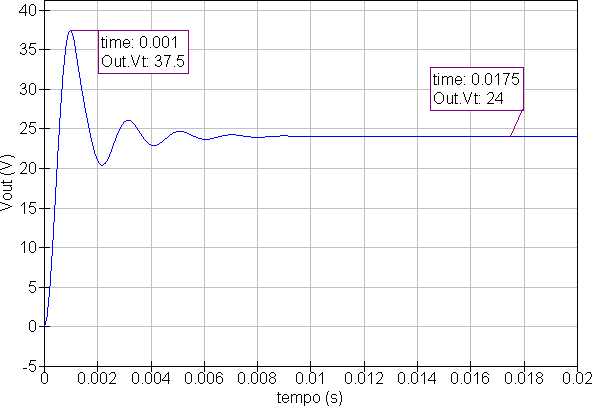
\includegraphics[width=0.8\textwidth]{vout_vinmax.png}
	\caption{Pico de tensão sobre a carga/capacitor.}
	\label{fig:vout_vinmax}
\end{figure}
\FloatBarrier
\item ESR máxima \\
Neste projeto, adotou-se 4\% como sendo o valor da máxima variação da corrente de saída (${\triangle}_{I_{out}}$). A Equação \ref{eq:esr_cap} apresenta o cálculo da resistência séria máxima do capacitor.

\begin{equation}
\label{eq:esr_cap}
\begin{split}
ESR & \leq \frac{{\triangle}_{V_{out}}}{{\triangle}_{I_{out}}} \\
& = \frac{4\%}{4\%} = 1 \Omega
\end{split}
\end{equation}

\end{enumerate}
% ---------------------------------------------
\item Indutor
\begin{enumerate}
\item Indutância \\
O cálculo para o valor mínimo da indutância (Equação \ref{eq:ind}) foi feito sobre o ponto onde o produto ($D \cdot V_{in}$) atinge seu valor máximo:

\begin{equation}
\label{eq:max_d_vin}
\begin{split}
max\left\{ D \cdot V_{in} \right\} & = max\left\{ \frac{(V_{out}-V_{in})}{V_{out} } \cdot V_{in} \right\} \\
& = max\left\{ \frac{(24-V_{in})}{24} \cdot V_{in} \right\} = 6 \rightarrow V_{in} = 12 \rightarrow D = 50\%
\end{split}
\end{equation}

\begin{equation}
\label{eq:ind}
\begin{split}
L & \geq \frac{D \cdot V_{in}}{{\triangle}_{I_{L}}\cdot f_{req}} \\
& = \frac{6}{{4\%}\cdot 250k} = 600 \mu H
\end{split}
\end{equation}

%\pagebreak

\item Corrente média \\
\label{subsub:corrente-media}
Através da simulação, obteve-se a corrente média que o indutor deve suportar (4,51A, quando $V_{in} = 9V$).

\begin{figure}[H]
	\centering
	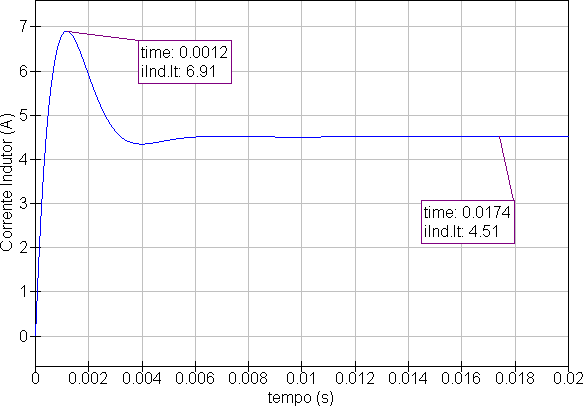
\includegraphics[width=0.67\textwidth]{iind_vinmin.png}
	\caption{Corrente média sobre o indutor.}
	\label{fig:iind_med}
\end{figure}
\pagebreak
\item Corrente máxima \\
\label{subsub:corrente-max}
Através da simulação, obteve-se a corrente máxima que o indutor deve suportar (8,22A, quando $V_{in} = 18V$).
\FloatBarrier
\begin{figure}[H]
	\centering
	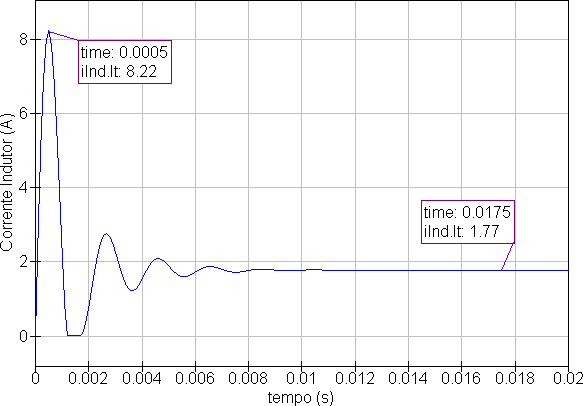
\includegraphics[width=0.67\textwidth]{iind_vinmax.png}
	\caption{Corrente máxima sobre o indutor.}
	\label{fig:iind_max}
\end{figure}
\FloatBarrier
\end{enumerate}
% ---------------------------------------------
\item Diodo
\begin{enumerate}
\item Corrente média e corrente máxima\\
A corrente no diodo é aproximadamente igual à corrente sobre a carga (desconsiderando os picos de carga sobre o capacitor). 
\FloatBarrier
\begin{figure}[H]
	\centering
	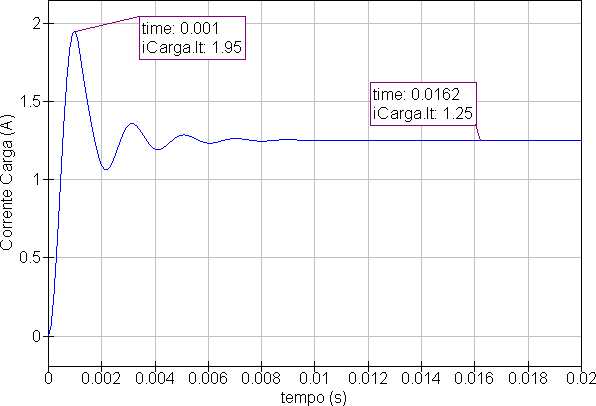
\includegraphics[width=0.7\textwidth]{icarga_vinmax.png}
	\caption{Corrente sobre o diodo/carga.}
	\label{fig:idiodo}
\end{figure}
\FloatBarrier
Através da simulação, obteve-se a corrente média e máxima que o diodo deve suportar (1,25A e 1,95, respectivamente, quando $V_{in} = 18V$).

\item Tensão reversa máxima \\
Através da simulação, obteve-se a máxima tensão reversa que o diodo deve suportar (35,6V, quando $V_{in} = 18V$).
\FloatBarrier
\begin{figure}[H]
	\centering
	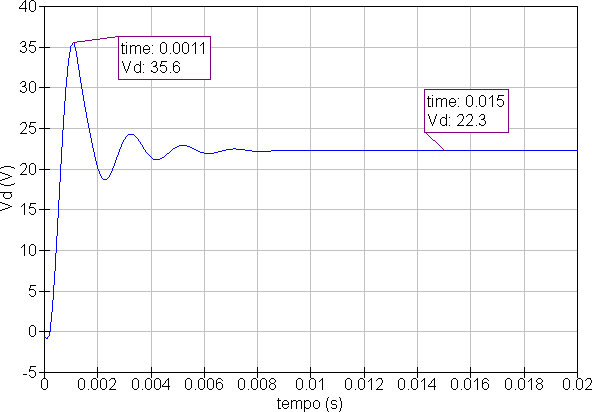
\includegraphics[width=0.62\textwidth]{vdrev_vinmax.png}
	\caption{Tensão reversa sobre o diodo.}
	\label{fig:vdrev}
\end{figure}
\FloatBarrier
\end{enumerate}
% ---------------------------------------------
\item Mosfet
\begin{enumerate}
\item Corrente média \\
Através da simulação, obteve-se a corrente média que a chave deve suportar (4,54A, quando $V_{in} = 9V$).
\FloatBarrier
\begin{figure}[H]
	\centering
	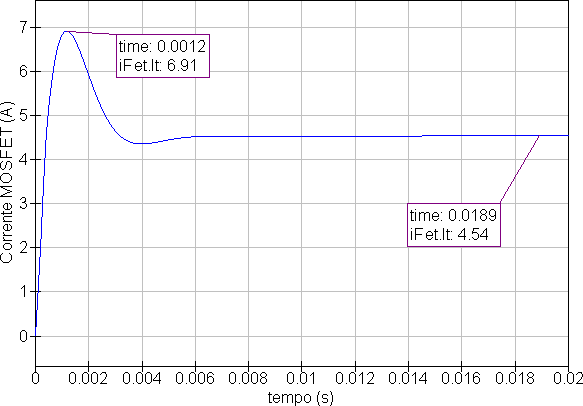
\includegraphics[width=0.62\textwidth]{ifet_vinmin.png}
	\caption{Corrente média sobre a chave.}
	\label{fig:ifet_med}
\end{figure}
\FloatBarrier
\pagebreak
\item Corrente máxima \\
Através da simulação, obteve-se a corrente máxima que a chave deve suportar (8,22A, quando $V_{in} = 18V$).
\FloatBarrier
\begin{figure}[H]
	\centering
	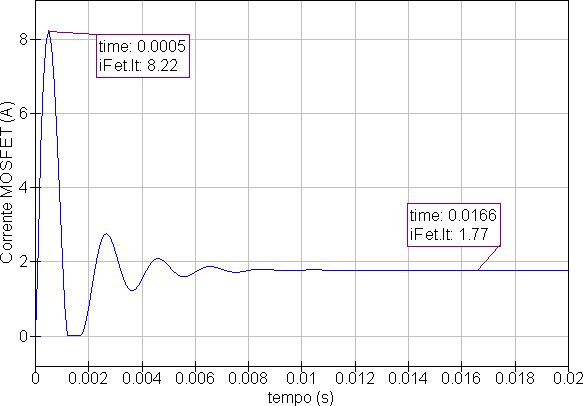
\includegraphics[width=0.67\textwidth]{ifet_vinmax.png}
	\caption{Corrente máxima sobre a chave.}
	\label{fig:ifet_max}
\end{figure}
\FloatBarrier
\item Tensão Dreno-Fonte
\label{subitem:vds}

Através da simulação, obteve-se a tensão máxima que a chave deve suportar (8,22V, quando $V_{in} = 18V$).

\begin{figure}[H]
	\centering
	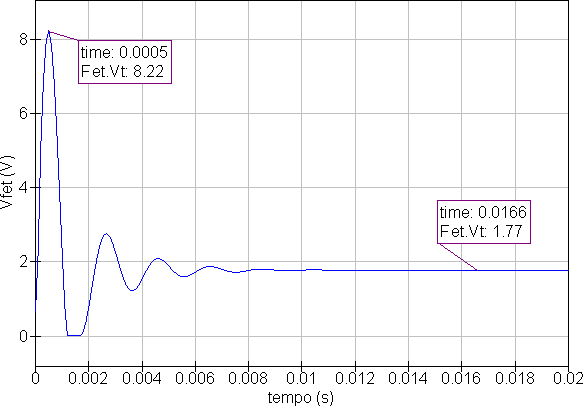
\includegraphics[width=0.67\textwidth]{vfet_vinmax.png}
	\caption{Tensão máxima sobre a chave.}
	\label{fig:vfet_max}
\end{figure}

\end{enumerate}

\end{enumerate}

\subsection*{Escolha dos componentes}
A partir dos dados obtidos através dos cálculos, da simulação e da disponibilidade, foram definidos os seguintes componentes:

\begin{enumerate}

\item Capacitor
\begin{itemize}
\item Fabricante: Nichicon
\item Part number: UVR1H470MED1TD
\item Capacitância: 2x$47 \mu F$ $\pm 20\%$ (2 em paralelo)
\item Tensão máxima de operação: 50V
\item ESR: não especificada pelo fabricante. Medida: $490 m\Omega$.
\end{itemize}

\item Diodo
\begin{itemize}
\item Fabricante: Vishay General Semiconductor
\item Part number: SB260
\item Queda de tensão: 680mV @ 2A
\item Corrente média: 2,0A
\item Pico máximo de corrente: 60A @ 8,3ms
\item Máxima tensão reversa: 60V
\end{itemize}

\item Mosfet
\begin{itemize}
\item Fabricante: Infineon Technologies	
\item Part number: IRFZ44EPBF
\item Corrente média: 48A
\item Pico máximo de corrente: 192A
\item Tensão máxima entre dreno e fonte: 60V
\item Resistência Dreno-Fonte modo triodo: $23m\Omega$ @$V_{GS} = 10V, I_D = 29A$
\item Tensão de limiar no \emph{gate}: 2V - 4V
\end{itemize}

\end{enumerate}

\clearpage

\section{Projeto do Indutor}

Para o cálculo do número de espiras do indutor em questão, foi utilizada a metodologia a partir do comprimento de entreferro. Assim, o carretel foi projetado de forma que o comprimento do entreferro fosse igual a 1,6mm, ou seja:

\begin{equation*}
\frac{l_g}{2} = 0,8mm
\end{equation*}

\begin{equation*}
N = \sqrt{\frac{l_g \cdot L}{\mu_0 \cdot A_e}} = \sqrt{\frac{1,6 \cdot 10^{-3} \cdot 600 \cdot 10^{-6}}{4 \cdot \pi \cdot 10^{-7} \cdot 1,7 \cdot 10^{-4}}} = 67,09\text{ espiras}
\end{equation*}

Onde:
\begin{itemize}
\item L - indutância [H]
\item $\mu_0$ - permeabilidade magnética do vácuo [H/m]
\item $A_e$ - área do núcleo [$m^2$]
\end{itemize}

Assim, utilizou-se 68 espiras para a construção do indutor. No entanto, é necessário verificar se a densidade de fluxo $B_{max}$ não ultrapassa o valor de 0,3T, provocando a saturação do núcleo. Como pode ser observado na Equação \ref{eq:b-max-erro}, não haverá saturação.

\begin{equation}
\label{eq:b-max-erro}
B_{max} =  \frac{L \cdot I_{pico}}{N \cdot A_e} = \frac{600 \cdot 10^{-6} \cdot 1,275}{68 \cdot 1,7 \cdot 10^{-4}} = 0,066T
\end{equation}

Foi então analisada a área disponível para o número de espiras calculado, pela equação abaixo, considerando a densidade de corrente máxima $J_{max}$ igual a $450 A/cm^2$ e a corrente eficaz $I_{ef}$ igual a 1,25 A.

\begin{equation}
\label{eq:area-erro}
A_{t} = \frac{I_{ef}}{J_{max}} = 0,0027 cm^2 = 0,27 mm^2
\end{equation}

No entanto, a corrente utilizada foi equivocada, uma vez que se considerou a corrente de saída média e não a corrente máxima que efetivamente passa pelo indutor em regime permanente. O erro foi identificado após a implementação do conversor e durante os ensaios, onde o indutor aqueceu. Refazendo os cálculos para verificar a dimensão do erro, utilizou-se a corrente máxima, na condição da tensão de entrada mínima, igual a 3,33 A:

\begin{equation}
\label{eq:area-erro}
A_{t} = \frac{I_{max}}{J_{max}} = 0,0074 cm^2 = 0,74 mm^2
\end{equation}

Dessa forma, seria necessária a utilização de um condutor $AWG_{18}$, cuja seção é de $0,82mm^2$.

Porém, como se está operando em frequência elevada para eletrônica de potência, deve-se considerar o efeito pelicular, utilizando a frequência do projeto igual a 250kHz.

\begin{equation*}
\triangle= \frac{7,5}{\sqrt{f}} = 0,015 cm = 0,15mm
\end{equation*}

Como o raio do condutor deve ser menor que $\triangle$, o condutor mais indicado seria o $AWG_{29}$, cujo raio é de 0,14295mm. No entanto, havia a disponibilidade do condutor $AWG_{30}$ e assim, seria necessária a utilização de um número de condutores em paralelo obtido pela equação:

\begin{equation*}
n_{cp} = \frac{AWG_{18}}{AWG_{30}} = 16,07 \approx 17 \text{ condutores em paralelo}
\end{equation*}

Assim, realizando os mesmos cálculos, porém com o valor da corrente média de saída, foi obtido um número de 3 condutores em paralelo utilizando o $AWG_{30}$, valor muito distante do necessário. Assim, o indutor foi construído com o condutor $AWG_{30}$ e 3 condutores em paralelo.

Após a construção do indutor, a medição de sua indutância indicou aproximadamente $643,7\mu H$. Além disso, a ESR medida foi igual a $480m\Omega$. (obs.: a Seção \ref{sec:conclusoes} aborda novamente o projeto do indutor).

\clearpage

\section{Projeto do Compensador}

\subsection{Circuito de Controle}

O compensador escolhido foi o do Tipo 3, cujo circuito e função transferência são apresentados nas Figuras \ref{fig:sch-comp} e \ref{fig:tf-comp}, respectivamente.

\begin{figure}[H]
	\centering
	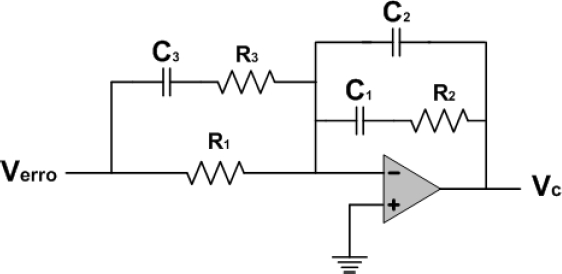
\includegraphics[width=0.4\textwidth]{sch-comp.jpg}
	\caption{Circuito do Compensador Tipo 3.}
	\label{fig:sch-comp}
\end{figure}

\begin{figure}[H]
	\centering
	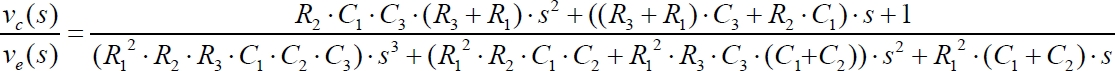
\includegraphics[width=0.98\textwidth]{tf-comp.jpg}
	\caption{Função transferência do Compensador Tipo 3.}
	\label{fig:tf-comp}
\end{figure}

A equação \ref{eq:tfboost} apresenta a função transferência do conversor \emph{Boost}.

\begin{equation}
\label{eq:tfboost}
\begin{split}
G_{Boost} ={\frac{V_{in}}{L \cdot C \cdot \left(1-D\right)^{2}}} \cdot \frac{ \left( - \frac{R_{SE} \cdot L \cdot C \cdot s^2}{R_0} + \left( R_{SE} \cdot C - \frac{L}{R_0} \right) \cdot s+1 \right) }{\left( s^2 + \left( \frac{1}{R_0 \cdot C} + \frac{R_{SE}}{L} \right) \cdot s + \frac{1}{L \cdot C} \right)}
\end{split}
\end{equation}

Onde
\begin{itemize}
\item \textbf{V\textsubscript{in}}: tensão de entrada
\item \textbf{L}: valor do Indutor \emph{Boost}
\item \textbf{C}: valor do Capacitor \emph{Boost}
\item \textbf{R\textsubscript{SE}}: ESR do capacitor
\item \textbf{R\textsubscript{0}}: carga do circuito
\item \textbf{D}: razão cíclica
\item \textbf{s}: variável no plano complexo (frequência complexa)
\end{itemize}

O projeto do compensador foi dado no ponto $Vin = 13,5V$. Assumindo esse valor na Equação \ref{eq:d_max_cap}, tem-se o valor da razão cíclica igual a $D = 0,4375$.

A fim de se obter valores mais próximos para o caso real, os componentes físicos foram medidos e o compensador foi projetado levando em conta esses valores.

\begin{itemize}
\item L = $643,7\mu H$
\item C = $2 \cdot 47\mu = 94\mu F$ (capacitores em paralelo)
\item R\textsubscript{SE} = $0,49 \Omega / 2 = 0,245 \Omega$ (capacitores em paralelo)
\item R\textsubscript{0} = $19,2 \Omega$
\end{itemize}

Com isso, obteve-se os diagramas de Bode em malha aberta, apresentados na Figura \ref{fig:bode}. Logo após, escolheu-se 2,08kHz para ser a frequência de corte em malha fechada, ponto onde a fase é de 166º (-194º) e magnitude é de 14dB (5,01V/V).

\begin{figure}[H]
	\centering
	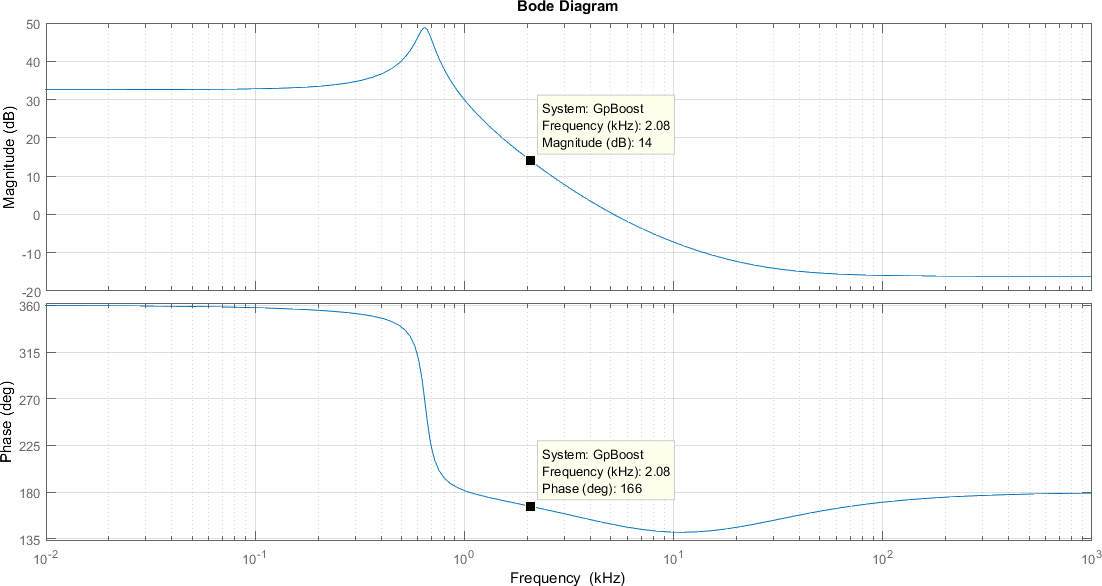
\includegraphics[width=0.98\textwidth]{GpBoost_freq_corte_escolhida.png}
	\caption{Diagramas de Bode da função transferência do conversor \emph{Boost}.}
	\label{fig:bode}
\end{figure}

Optou-se pela margem de fase igual a 60º. Com isso, obteve-se o avanço de fase, conforme a Equação \ref{eq:avanco-fase}.

\begin{equation}
\label{eq:avanco-fase}
\begin{split}
\phi_{\text{avanço}} & = -90^{\circ} + MF_{desejada} - \angle G_{Boost}\mid_{f_c} \\
& = -90^{\circ} + 60^{\circ} - (-194^{\circ}) = 164^{\circ}
\end{split}
\end{equation}

O ganho do compensador deve ser tal que leve a um ganho unitário em malha fechada, na frequência de corte (Equação \ref{eq:ganho-unit}).

\begin{equation}
\label{eq:ganho-unit}
\begin{split}
\mid G_{FTMA}\left(s\right)\mid_{f_c} = \mid G_{C}\left(s\right)\mid_{f_c} \cdot \mid G_{PWM}\left(s\right)\mid_{f_c} \cdot \mid G_{Boost}\left(s\right)\mid_{f_c} \cdot k = 1
\end{split}
\end{equation}

Substituindo os seguintes valores na Equação \ref{eq:ganho-unit}, obteve-se o \text{Ganho do Compensador} $\mid G_c\left( s \right) \mid_{f_c} = 1,7957V/V$.

\begin{itemize}

\item \text{Ganho da planta do conversor}: $ \mid G_{Boost} \left( s \right) \mid_{f_c} = 5,01$

\item \text{Ganho da modulação PWM}: $\mid G_{PWM}\left( s \right) \mid_{f_c} = 1/V_{triang} = 1/1,8 = 0,5556$

\item \text{Ganho do divisor resistivo de \emph{feedback}}: $ k = 5V / 24V = 0,2 $

\end{itemize}

O fator $k_{pz}$ é dado pela Equação \ref{eq:kpz}.

\begin{equation}
\label{eq:kpz}
\begin{split}
k_{pz} & = \left( \tan \left( \frac{\phi_{\text{avanço}}}{4}+\frac{\pi}{4} \right)  \right)^2 \\
& = \left( \tan \left( \frac{164}{4}+\frac{\pi}{4} \right)  \right)^2 = 204,5091
\end{split}
\end{equation}

Tomando o resistor $R_1 = 510k\Omega$, calculou-se os demais componentes do compensador.

\begin{equation}
\label{eq:comp-c2}
\begin{split}
C_{2} & = \frac{1}{2 \cdot \pi \cdot f_{c} \cdot R_{1} \cdot \mid G_{c} \left( s \right)\mid} \\
& = \frac{1}{2 \cdot \pi \cdot 2,08kHz \cdot 510k\Omega \cdot 1,7957} = 83,550pF
\end{split}
\end{equation}

\begin{equation}
\label{eq:comp-c1}
\begin{split}
C_{1} & = C_{2} \cdot \left( k_{pz}-1 \right) \\
& =  83,550pF \cdot \left( 204,5091 - 1 \right) = 17nF
\end{split}
\end{equation}

\begin{equation}
\label{eq:comp-r2}
\begin{split}
R_{2} & = \frac{\sqrt{k_{pz}}}{2 \cdot \pi \cdot f_{c} \cdot C_{1}} \\
& = \frac{\sqrt{204,5091}}{2 \cdot \pi \cdot 2,08k\Omega \cdot 17nF} = 64,355k\Omega
\end{split}
\end{equation}

\begin{equation}
\label{eq:comp-r3}
\begin{split}
R_{3} & = \frac{R_{1}}{k{pz}-1} \\
& = \frac{510k\Omega}{204,5091-1} = 2,51k\Omega
\end{split}
\end{equation}

\begin{equation}
\label{eq:comp-c3}
\begin{split}
C_{3} & = \frac{1}{2 \cdot \pi \cdot f_{c} \cdot R_{3} \cdot \sqrt{k_{pz}}} \\
& = \frac{1}{2 \cdot \pi \cdot 2,08kHz \cdot 2,51k\Omega \cdot \sqrt{204,5091}} = 2,14nF
\end{split}
\end{equation}

Após os cálculos, foi feita uma aproximação com valores comerciais e/ou disponíveis, através de arranjos série/paralelo, obtendo aos seguintes valores:

\begin{table}[H]
\centering
\caption{aproximação com valores comerciais/disponíveis}
\label{tab:comp-com}
\begin{tabular}{ll}
$R_1 \left( k\Omega \right)$ & 510 \\
$R_2 \left( k\Omega \right)$ & 56 \\
$R_3 \left( k\Omega \right)$ & 2,2 \\
$C_1 \left( nF \right)$ & 17,2 \\
$C_2 \left( pF \right)$ & 94 \\
$C_3 \left( nF \right)$ & 2,2
\end{tabular}
\end{table}

Substituindo as devidas funções transferências no sistema da Figura \ref{fig:sistema-controle}, obteve-se os diagramas de Bode da Figura \ref{fig:bode-controle}.

\begin{figure}[H]
	\centering
	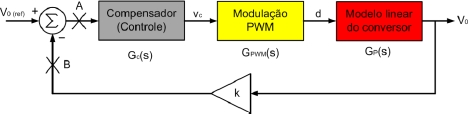
\includegraphics[width=0.9\textwidth]{sistema-controle.jpg}
	\caption{Sistema de controle do conversor \emph{Boost}.}
	\label{fig:sistema-controle}
\end{figure}

\begin{figure}[H]
	\centering
	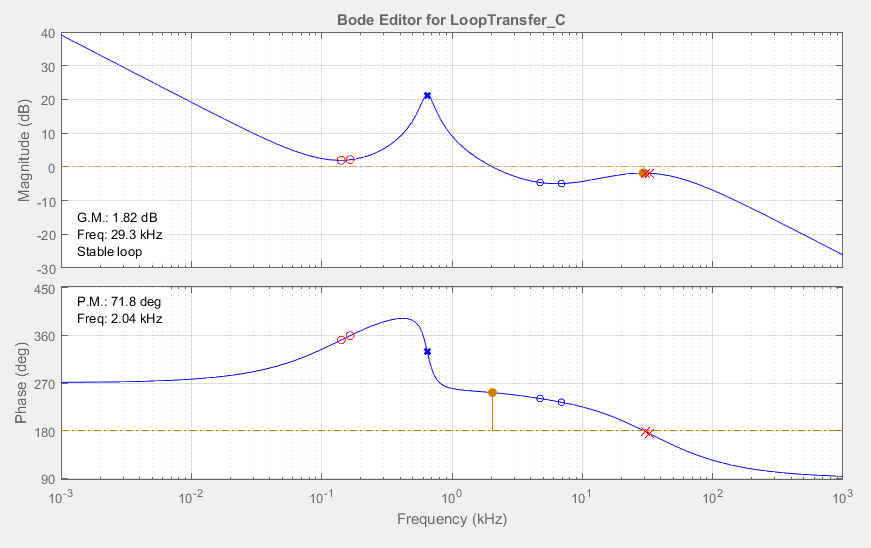
\includegraphics[width=0.99\textwidth]{CompensadorBode.png}
	\caption{Diagramas de Bode do conversor \emph{Boost}.}
	\label{fig:bode-controle}
\end{figure}

\subsection{Frequência de Oscilação}

A implementação do compensador foi realizada através do circuito integrado TL494, cujo diagrama simplificado é apresentado na Figura \ref{fig:tl494}.

\begin{figure}[H]
	\centering
	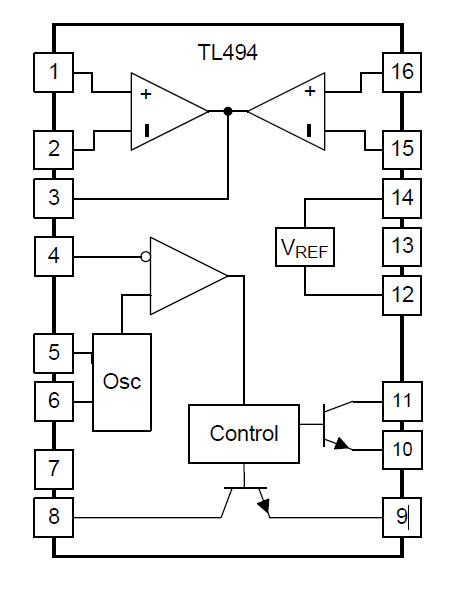
\includegraphics[width=0.35\textwidth]{diag-simp.PNG}
	\caption{Diagrama simplificado do CI TL494.}
	\label{fig:tl494}
\end{figure}

Segundo sua documentação (\emph{datasheet}), a frequência de oscilação é dada pelo inverso do produto de um capacitor ($C_T$) e um resistor ($R_T$), conectados aos pinos 5 e 6, respectivamente. O cálculo para $f_{OSC} \approx 250kHz$ é apresentado na Equação \ref{eq:fosc}.
\begin{equation}
\label{eq:fosc}
\begin{split}
f_{OSC} & = \frac{1}{C_T \cdot R_T} \\
& = \frac{1}{1,8nF \cdot 2,2k\Omega} = 253kHz
\end{split}
\end{equation}

\subsection{Tensão de \emph{feedback}}

A entrada não-inversora do comparador (pino 1) recebe a tensão de \emph{feedback} do conversor \emph{Boost}, devendo ser ajustada à faixa 0V - 5V. Para isso, implementou-se um divisor resistivo, apresentado na Equação \ref{eq:div-res}.

\begin{equation}
\label{eq:div-res}
\begin{split}
V_{feedback_{max}} & = \frac{24V \cdot 1k\Omega}{1k\Omega + 3,8k\Omega}  = 5V
\end{split}
\end{equation}

\subsection{\emph{Soft-start} e tempo-morto}

As técnicas de \emph{soft-start} e tempo-morto são necessárias para mitigar o estresse sobre o \emph{Mosfet} durante a inicialização do sistema, fazendo com que o capacitor \emph{Boost} se carregue lentamente. A Figura \ref{fig:soft-start} apresenta a limitação do ciclo de trabalho em função da tensão aplicada no pino 4 do circuito integrado.

\begin{figure}[H]
	\centering
	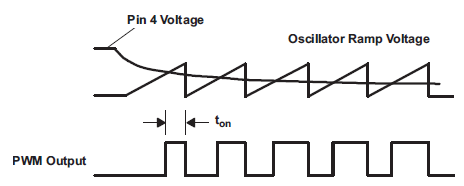
\includegraphics[width=0.65\textwidth]{soft-start.PNG}
	\caption{Controle do ciclo de trabalho.}
	\label{fig:soft-start}
\end{figure}

A entrada do comparador do tempo-morto (pino 4) trabalha com tensões entre 0V e 3,3V, fazendo com que o \emph{Mosfet} seja cortado, proporcionalmente, de 3\% a 100\%, ou seja, a razão cíclica varia entre 0,97 e 0.

A Equação \ref{eq:deadv} apresenta o cálculo para a máxima tensão no pino 4 em função do máximo valor da razão cíclica (escolhido $D = 85\%$).

\begin{equation}
\label{eq:deadv}
\begin{split}
V_{4_{max}} & = \frac{3,3V \cdot \left(0,97-0,85\right)}{0,97} = 0,408V
\end{split}
\end{equation}

Como pode ser notado na Figura \ref{fig:soft-div}, a tensão interna de referência é de 5V, sendo necessário um divisor resistivo para limitar o pino 4 em 0,408V. Assumindo o resistor \emph{shunt} igual a $10k\Omega$, tem-se o seguinte valor do resistor $R_{T_{ss}}$ (Equação \ref{eq:soft-div-res}).

\begin{figure}[H]
	\centering
	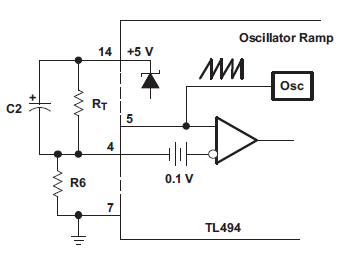
\includegraphics[width=0.5\textwidth]{soft-div.png}
	\caption{Circuito de \emph{soft-start}.}
	\label{fig:soft-div}
\end{figure}

\begin{equation}
\label{eq:soft-div-res}
\begin{split}
R_{T_{ss}} & = R_{shunt} \cdot \left( \frac{V_{ref}}{V_{4_{max}}} - 1\right) \\
& = 10k\Omega \cdot \left( \frac{5V}{0,408V} - 1\right) \approx 110k\Omega
\end{split}
\end{equation}

Para o tempo de \emph{soft-start}, definiu-se o equivalente para 93 ciclos de \emph{clock}, assim, o valor da capacitância é dada pela Equação \ref{eq:soft-cap}.

\begin{equation}
\label{eq:soft-cap}
\begin{split}
C_{ss} & =  \frac{1}{f_{OSC}} \cdot \frac{N_{ciclos}}{R_{T_{ss}}}\\
& = \frac{1}{250kHz} \cdot \frac{93}{110k\Omega} \approx 3,3nF
\end{split}
\end{equation}

A Figura \ref{fig:sch-controle} apresenta o circuito de controle/compensação completo.

\begin{figure}[H]
	\centering
	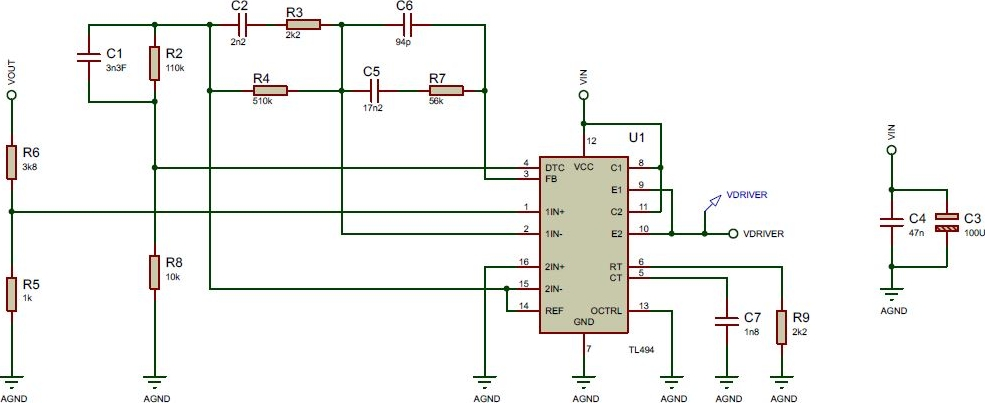
\includegraphics[width=1.0\textwidth]{sch-controle.jpg}
	\caption{Circuito de controle/compensação.}
	\label{fig:sch-controle}
\end{figure}


\clearpage

\section{Placa de Circuito Impresso}

A placa de circuito impresso foi projetada com base em boas práticas de leiaute e alguns cuidados foram tomados em relação à disposição dos circuitos.
\\
\\
O circuito de potência (Figura \ref{fig:sch-pot}) foi projetado com trilhas largas e buscou-se fazê-lo com o menor \emph{loop} possível. Ademais, para diminuir os efeitos da ESR, o capacitor Boost de $78,125\mu F$ foi substituído por 2 capacitores (CB1 e CB2) de $47\mu F$ em paralelo, totalizando $\approx100\mu F$ e metade da ESR inicial ($490 m\Omega/2=245m\Omega$).

\begin{figure}[H]
	\centering
	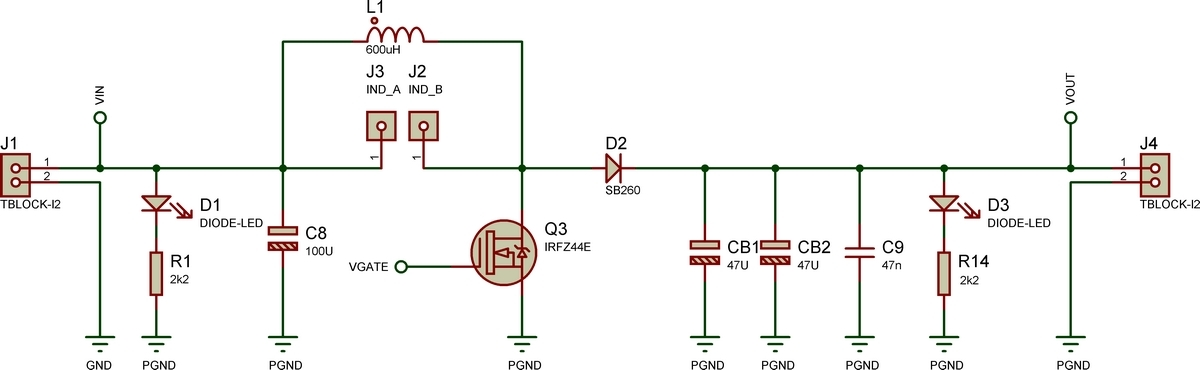
\includegraphics[width=0.95\textwidth]{sch-potencia.jpg}
	\caption{Esquemático do circuito de potência.}
	\label{fig:sch-pot}
\end{figure}

Para evitar que ruídos provenientes dos circuitos de potência (Figura \ref{fig:sch-pot}) e de chaveamento (Figura \ref{fig:sch-chaveamento}) interferissem no circuito de controle (Figura \ref{fig:sch-controle}), separou-se os terras através de componentes virtuais \emph{neckties}, como apresentado na Figura \ref{fig:neckties}. Dessa forma, cada circuito é tratado de forma individual, tendo a ligação das referências próxima ao conector de entrada (Figura \ref{fig:plano-baixa}).

\begin{figure}[H]
	\centering
	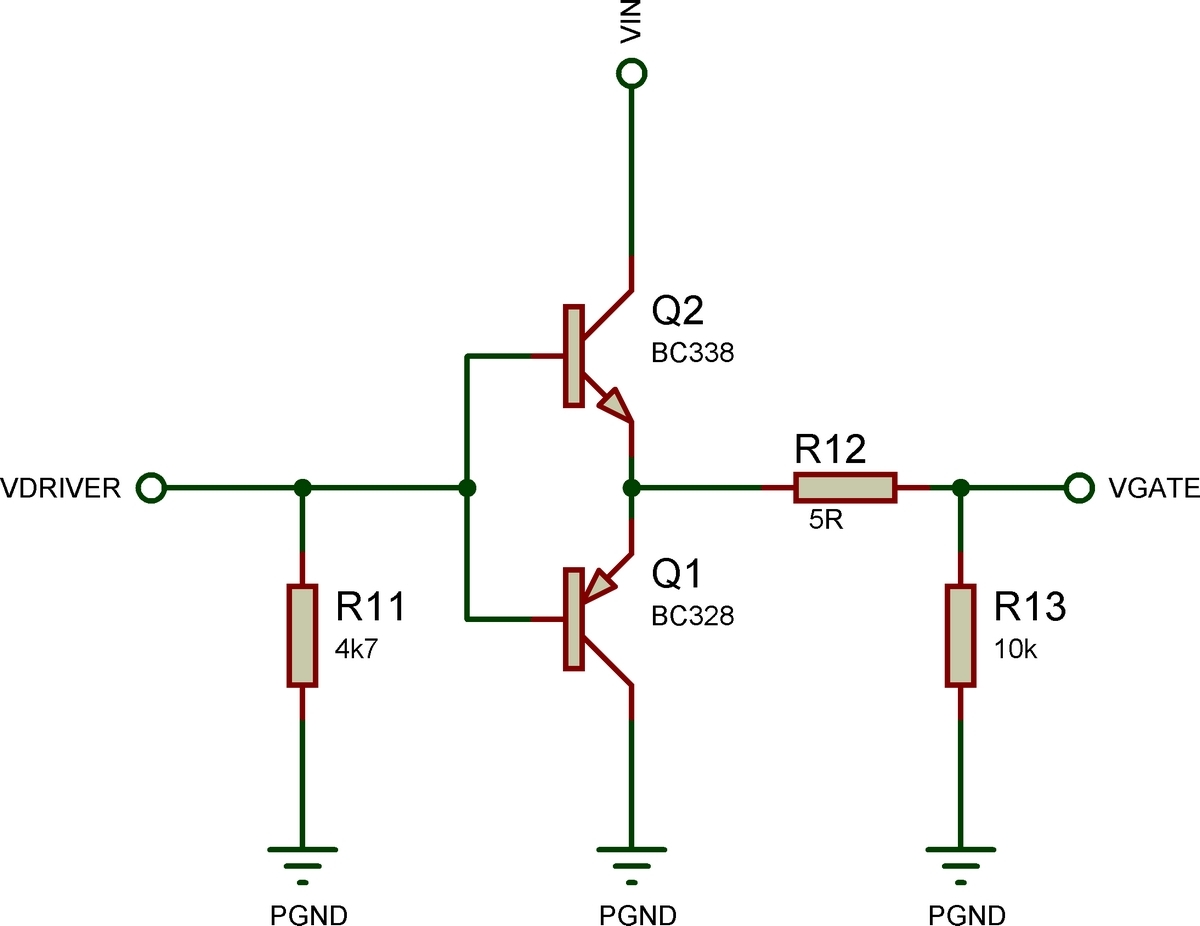
\includegraphics[width=0.5\textwidth]{sch-acionamento.jpg}
	\caption{Esquemático do circuito de chaveamento.}
	\label{fig:sch-chaveamento}
\end{figure}

\begin{figure}[H]
	\centering
	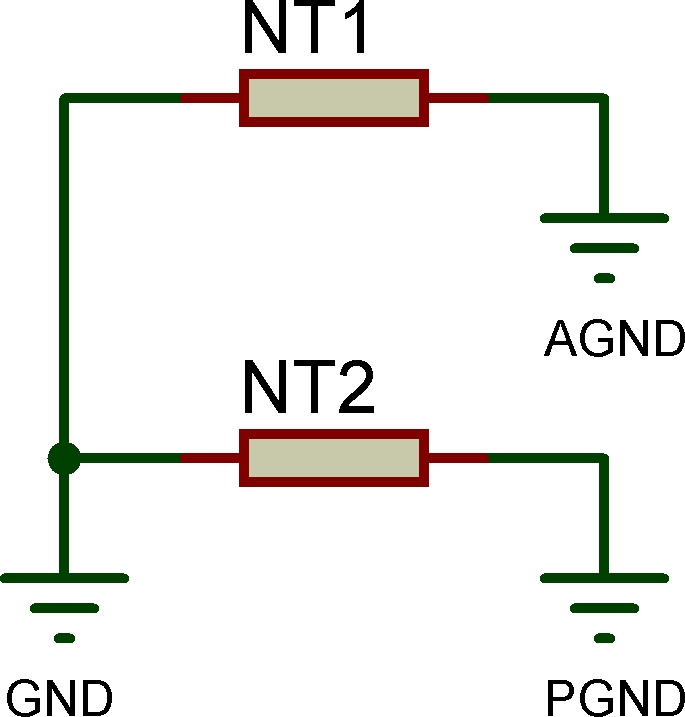
\includegraphics[width=0.28\textwidth]{sch-gnds.jpg}
	\caption{Separação dos terras de alta (PGND) e baixa (AGND) potência.}
	\label{fig:neckties}
\end{figure}

Além disso, o circuito de controle foi confinado em um pequeno plano de terra individual, como apresentado na Figura \ref{fig:plano-baixa}.

\begin{figure}[H]
	\centering
	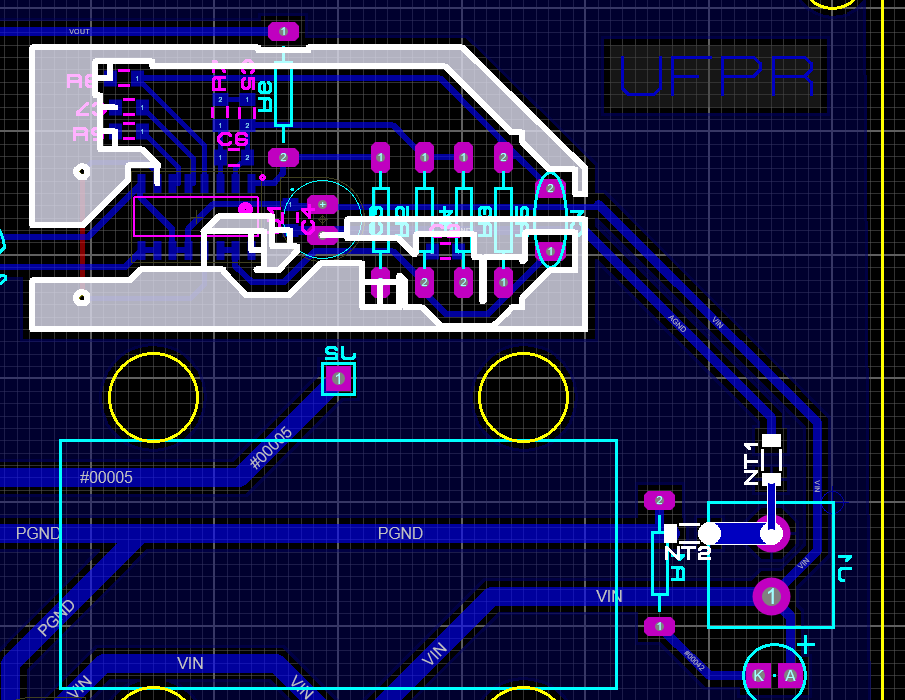
\includegraphics[width=0.82\textwidth]{pcb-ground-plane-net-tail.png}
	\caption{Destaque do plano confinado e \emph{neckties} na entrada do circuito separando os terras.}
	\label{fig:plano-baixa}
\end{figure}

Com o circuito de controle estando afastado do conector de entrada, foram colocados 2 capacitores de desacoplamento próximos ao CI TL494.

\begin{figure}[H]
	\centering
	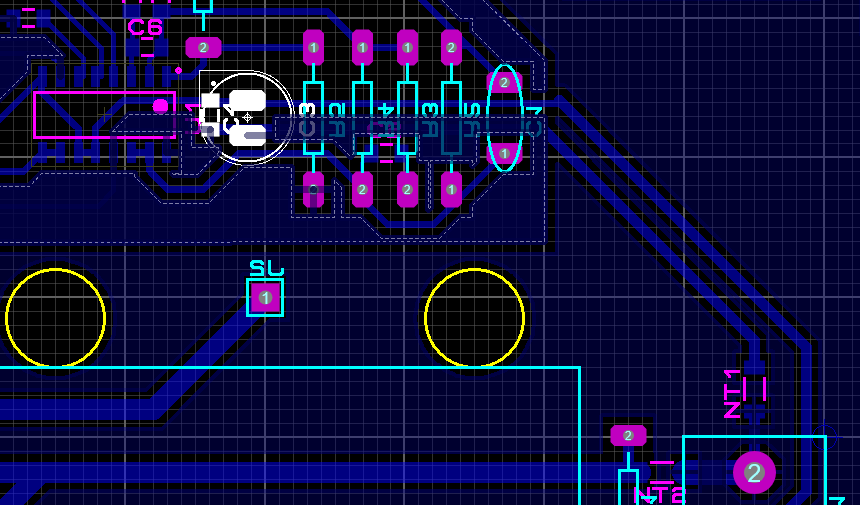
\includegraphics[width=0.82\textwidth]{pcb-caps-desacopl.png}
	\caption{Destaque dos capacitores de desacoplamento próximos ao circuito integrado.}
	\label{fig:caps-des}
\end{figure}

A Figura \ref{fig:pcb-layout} apresenta o leiaute completo e as Figuras \ref{fig:3d-top} e \ref{fig:3d-bot} apresentam as vistas superior e inferior do modelo 3D, respectivamente. Em seguida, a Figura \ref{fig:top-confec} mostra o protótipo construído.

\begin{figure}[H]
	\centering
	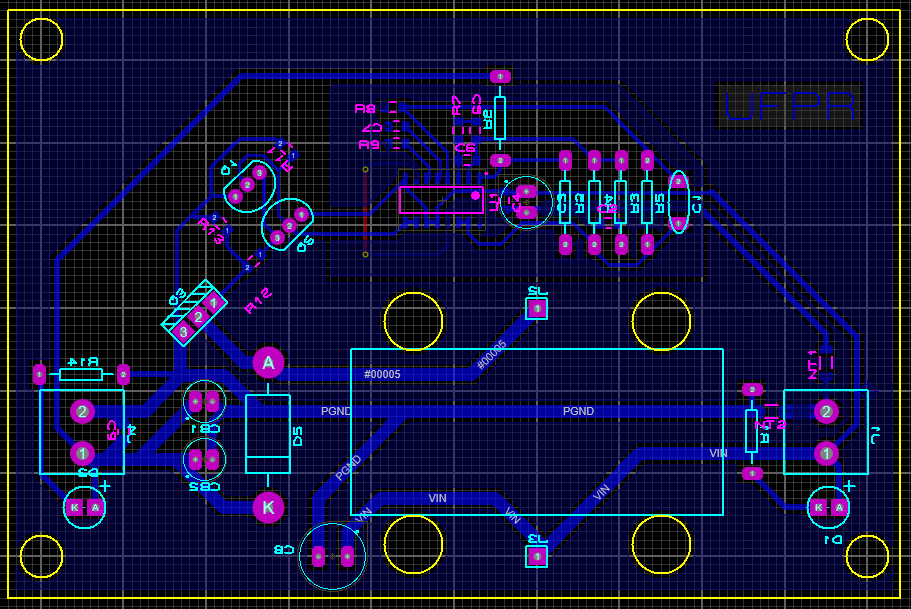
\includegraphics[width=0.87\textwidth]{pcb-layout.png}
	\caption{Leiaute da placa de circuito impresso.}
	\label{fig:pcb-layout}
\end{figure}

\begin{figure}[H]
	\centering
	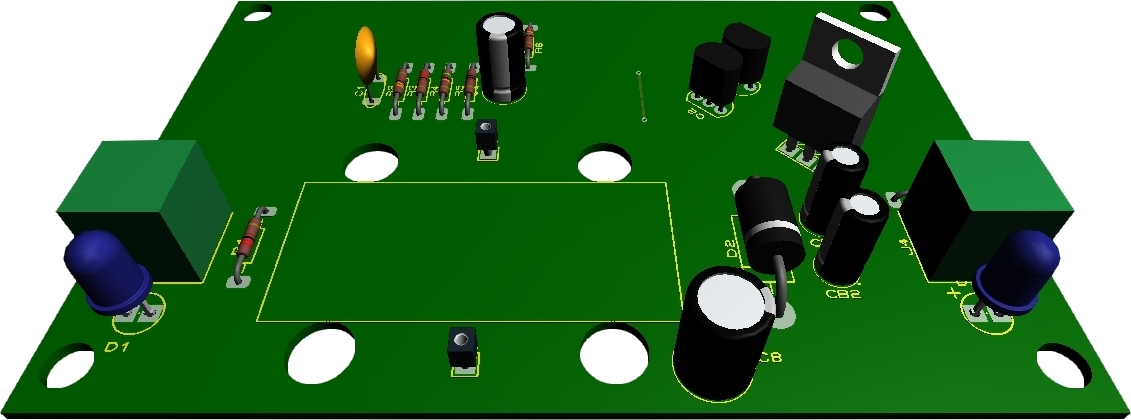
\includegraphics[width=0.87\textwidth]{3d-top.jpg}
	\caption{Vista superior do modelo 3D.}
	\label{fig:3d-top}
\end{figure}

\begin{figure}[H]
	\centering
	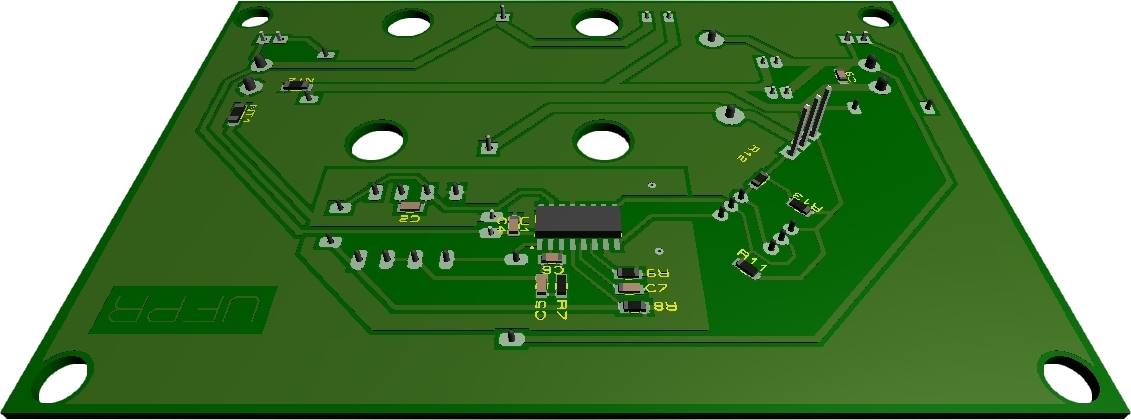
\includegraphics[width=0.9\textwidth]{3d-bottom.jpg}
	\caption{Vista inferior do modelo 3D.}
	\label{fig:3d-bot}
\end{figure}

\begin{figure}[H]
	\centering
	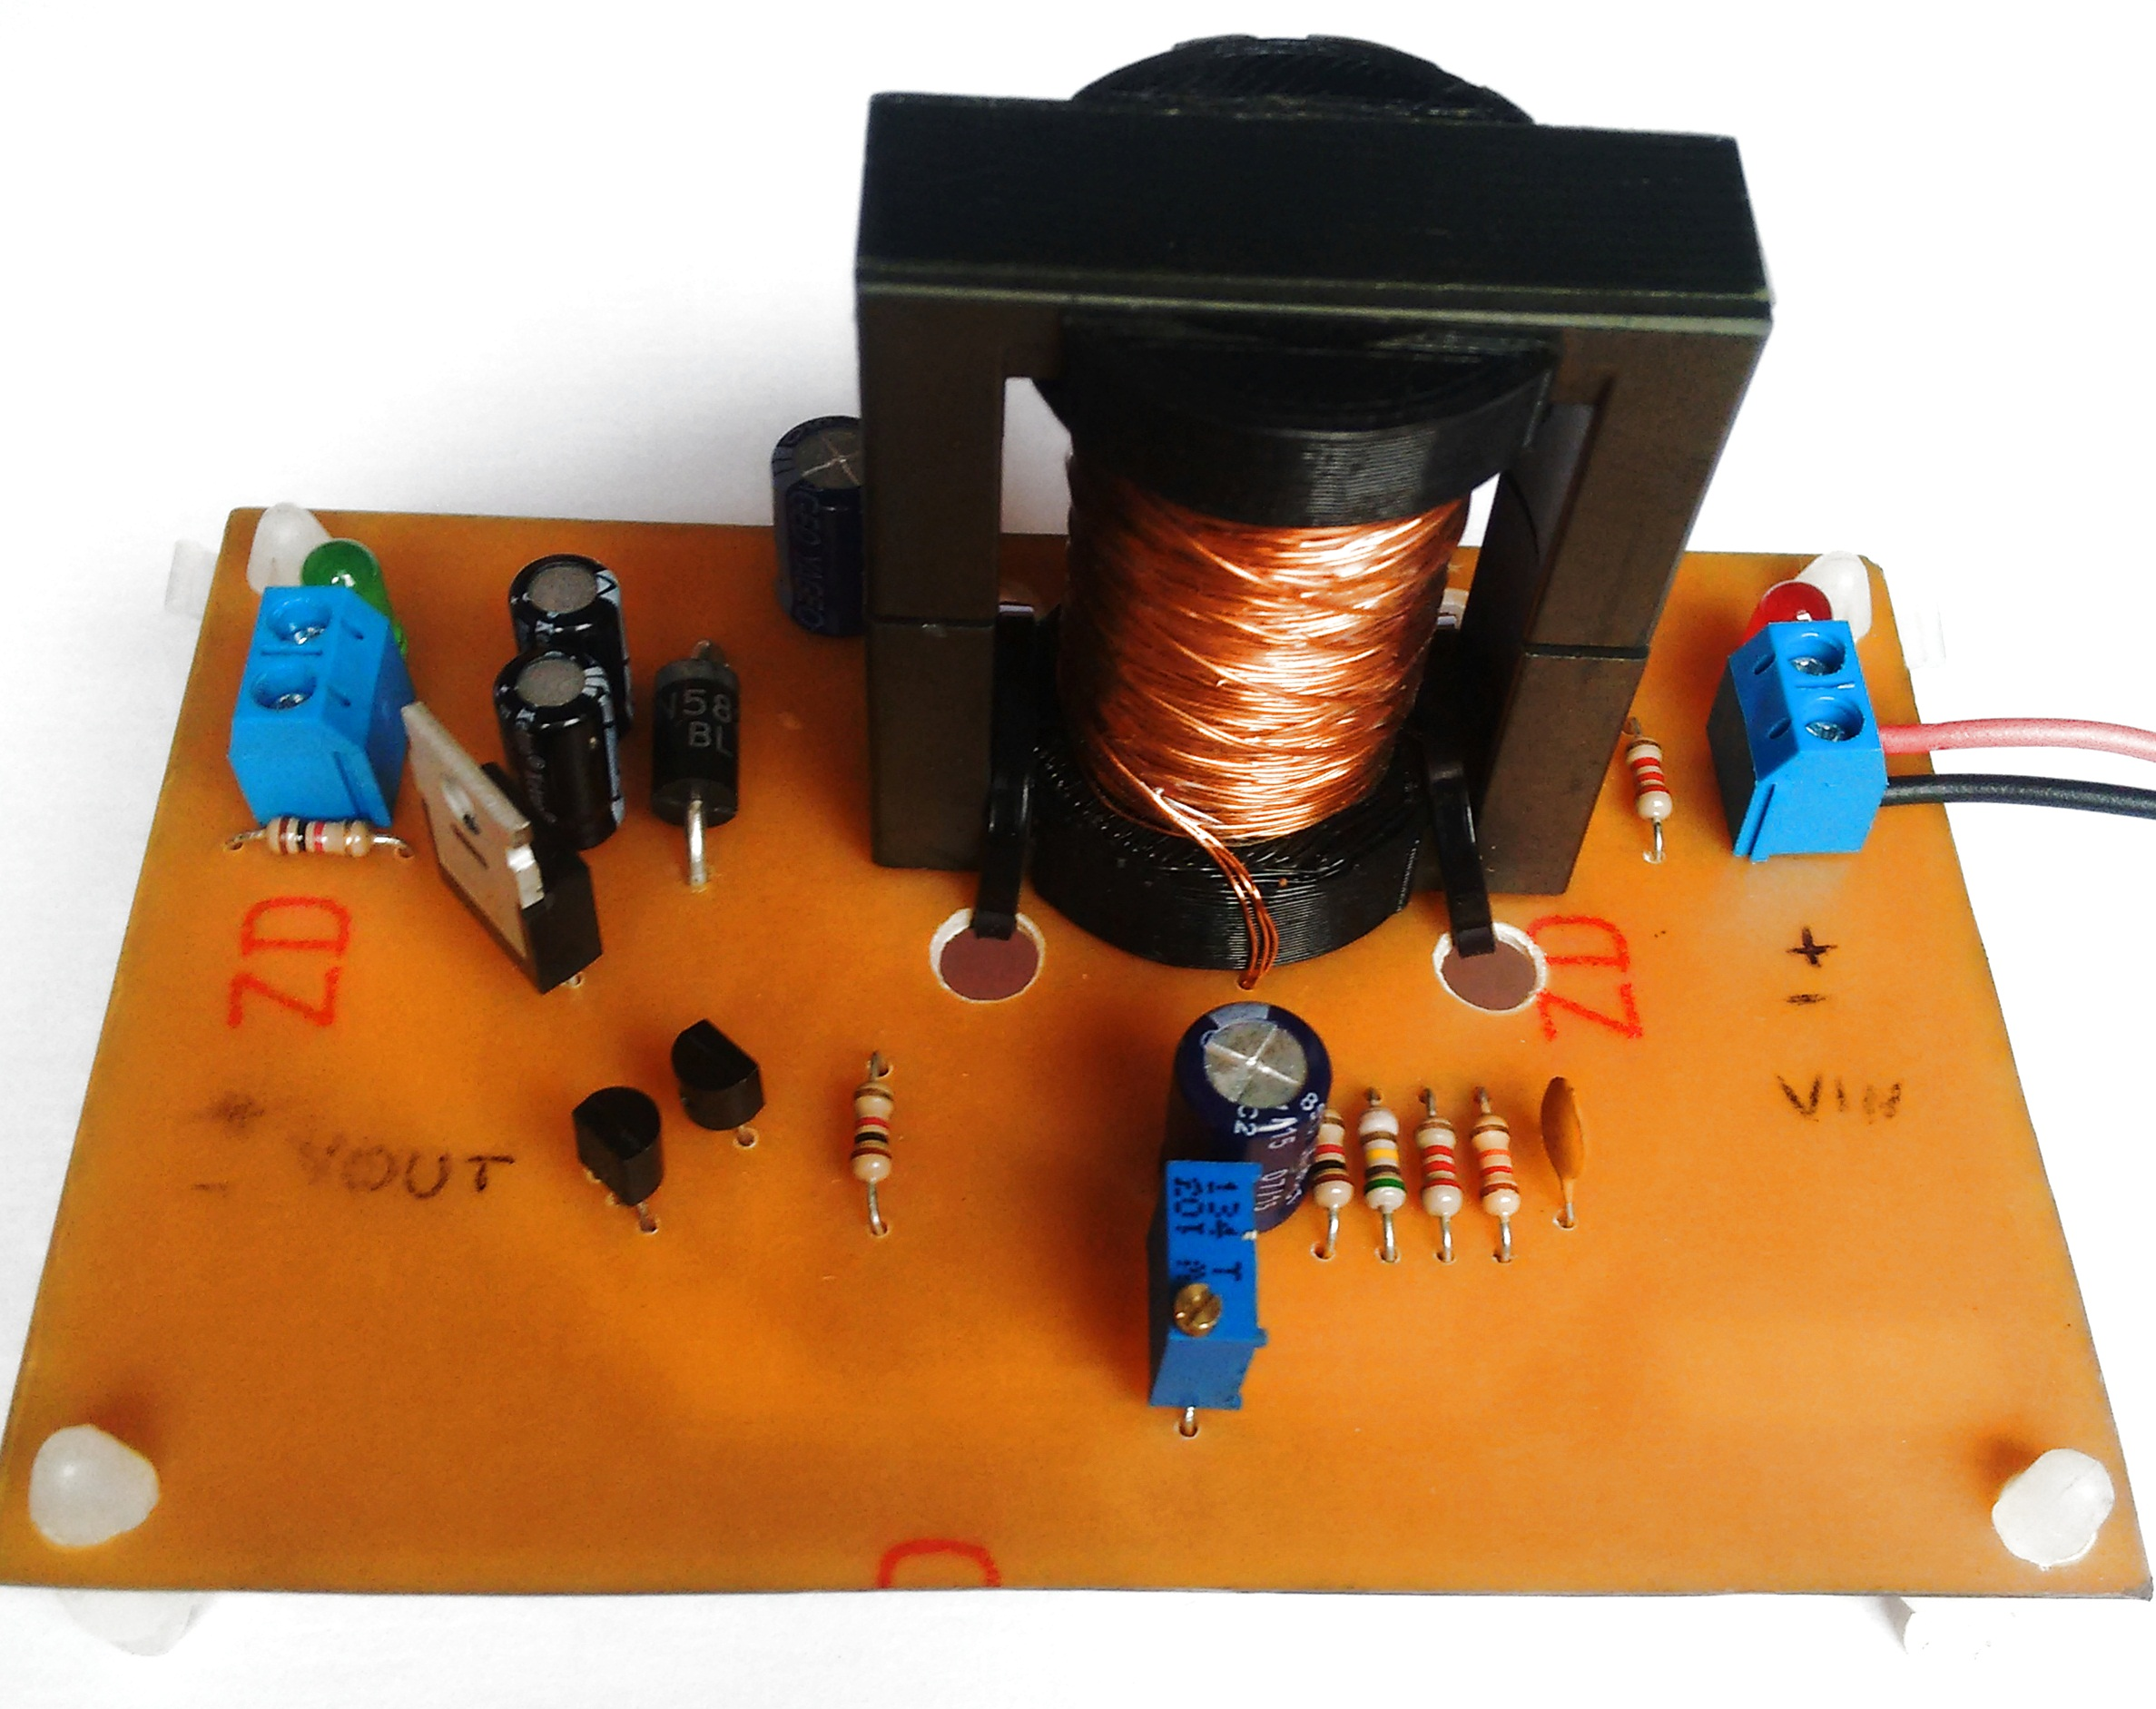
\includegraphics[width=0.75\textwidth]{c2.jpg}
	\caption{Vista superior do protótipo confeccionado.}
	\label{fig:top-confec}
\end{figure}

\clearpage

%\section{Simulação do Conversor \textit{Boost}}
%\clearpage

\section{Resultados}
\label{sec:resultados}

Os parâmetros analisados foram obtidos em 3 pontos bem definidos sobre a faixa de operação: 9V, 13,5V e 18V.

\subsection{Ondulação da tensão de saída}

As Figuras \ref{fig:ripple-18V}, \ref{fig:ripple-13v5} e \ref{fig:ripple-9V} apresentam o \emph{ripple} (ondulação) da tensão de saída para os 3 casos citados, com carga de 30W.
\FloatBarrier
\begin{figure}[H]
	\centering
	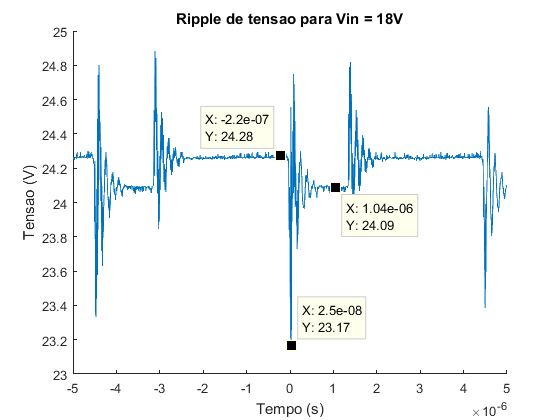
\includegraphics[width=0.8\textwidth]{ripple-vin-18V.png}
	\caption{\emph{Ripple} da tensão de saída @Vin=18V.}
	\label{fig:ripple-18V}
\end{figure}
\FloatBarrier
\begin{figure}[H]
	\centering
	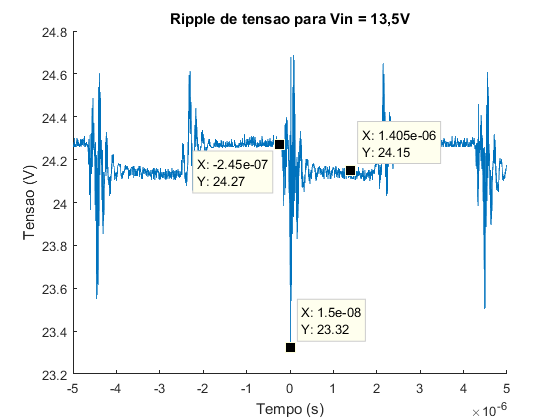
\includegraphics[width=0.8\textwidth]{ripple-vin-13V5.png}
	\caption{\emph{Ripple} da tensão de saída @Vin=13,5V.}
	\label{fig:ripple-13v5}
\end{figure}
\FloatBarrier
\begin{figure}[H]
	\centering
	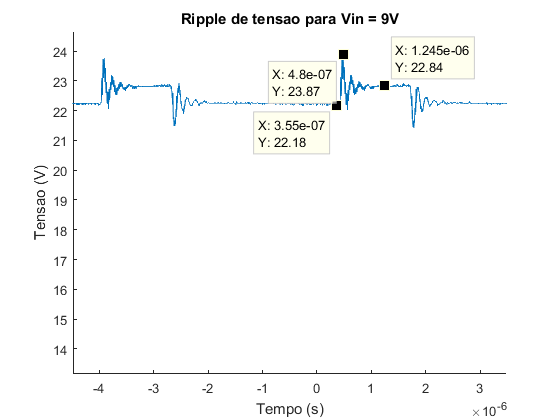
\includegraphics[width=0.8\textwidth]{ripple-vin-9V.png}
	\caption{\emph{Ripple} da tensão de saída @Vin=9V.}
	\label{fig:ripple-9V}
\end{figure}
\FloatBarrier
\subsection{Transitório para o aumento da carga}

Para esta análise, alterou-se a carga de 15W ($2 \cdot R_{Carga}~=~38,4\Omega$) para 30W ($R_{Carga} = 19,2\Omega$). As Figuras \ref{fig:trans-2R-R-18V}, \ref{fig:trans-2R-R-13V5} e \ref{fig:trans-2R-R-9V} apresentam a oscilação da tensão de saída em função da alteração brusca (degrau) da carga.

\begin{figure}[H]
	\centering
	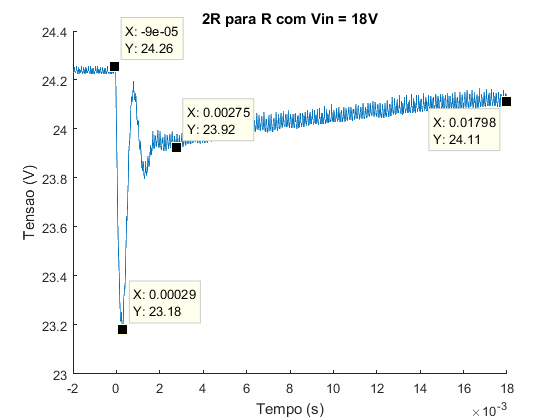
\includegraphics[width=0.8\textwidth]{2R-para-R-18V.png}
	\caption{Oscilação da tensão de saída devido a alteração brusca da carga @Vin=18V.}
	\label{fig:trans-2R-R-18V}
\end{figure}

\begin{figure}[H]
	\centering
	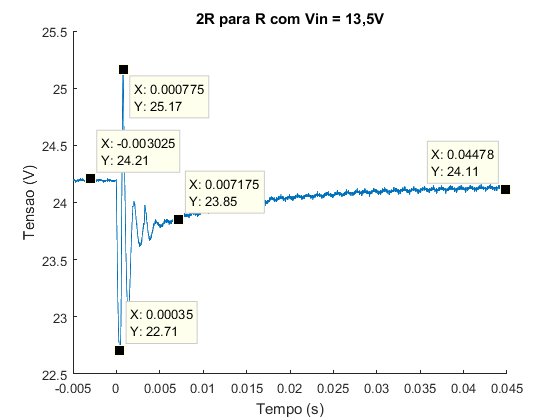
\includegraphics[width=0.8\textwidth]{2R-para-R-13V5.png}
	\caption{Oscilação da tensão de saída devido a alteração brusca da carga @Vin=13V5.}
	\label{fig:trans-2R-R-13V5}
\end{figure}

\begin{figure}[H]
	\centering
	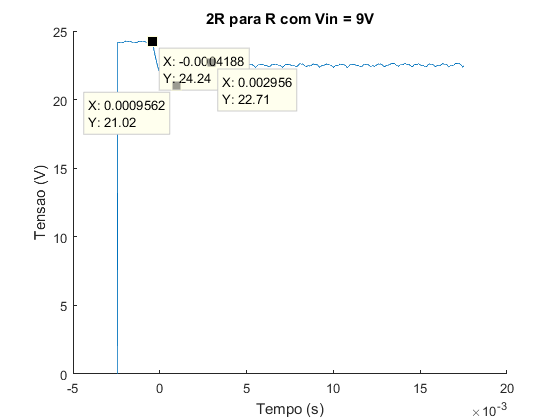
\includegraphics[width=0.8\textwidth]{2R-para-R-9V.png}
	\caption{Oscilação da tensão de saída devido a alteração brusca da carga @Vin=9V.}
	\label{fig:trans-2R-R-9V}
\end{figure}


\subsection{Transitório para a diminuição da carga}

Similar ao caso anterior, alterou-se a carga de 30W ($R_{Carga} = 19,2\Omega$) para 15W ($2 \cdot R_{Carga}~=~38,4\Omega$). As Figuras \ref{fig:trans-R-2R-18V}, \ref{fig:trans-R-2R-13V5} e \ref{fig:trans-R-2R-9V} apresentam a oscilação da tensão de saída em função da alteração brusca (degrau) da carga.

\begin{figure}[H]
	\centering
	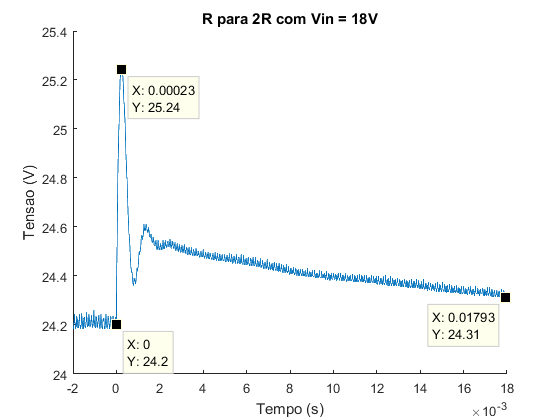
\includegraphics[width=0.8\textwidth]{R-para-2R-18V.png}
	\caption{Oscilação da tensão de saída devido a alteração brusca da carga @Vin=18V.}
	\label{fig:trans-R-2R-18V}
\end{figure}

\begin{figure}[H]
	\centering
	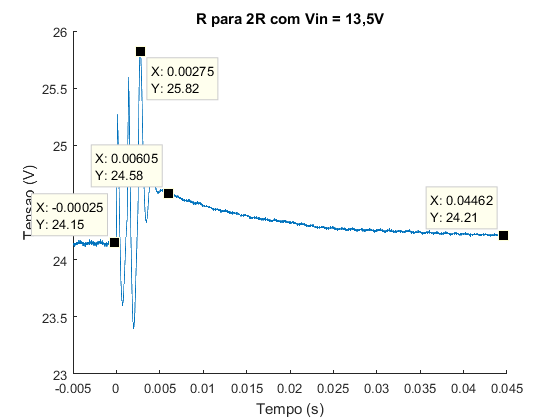
\includegraphics[width=0.8\textwidth]{R-para-2R-13V5.png}
	\caption{Oscilação da tensão de saída devido a alteração brusca da carga @Vin=13V5.}
	\label{fig:trans-R-2R-13V5}
\end{figure}

\begin{figure}[H]
	\centering
	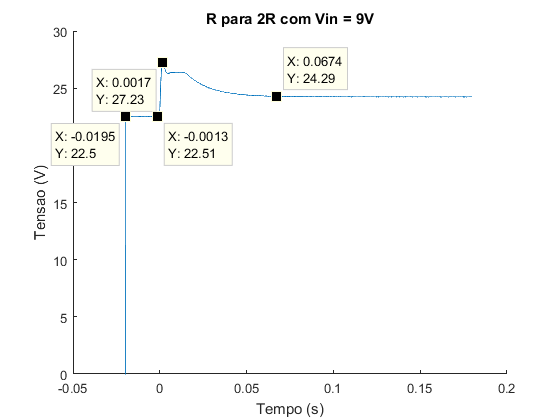
\includegraphics[width=0.8\textwidth]{R-para-2R-9V.png}
	\caption{Oscilação da tensão de saída devido a alteração brusca da carga @Vin=9V.}
	\label{fig:trans-R-2R-9V}
\end{figure}

\subsection{Tensão dreno-fonte}
\label{subsub:vds}

As Figuras \ref{fig:vds-18V}, \ref{fig:vds-13V5} e \ref{fig:vds-9V} apresentam a tensão dreno-fonte do Mosfet, também para os 3 casos citados.

\begin{figure}[H]
	\centering
	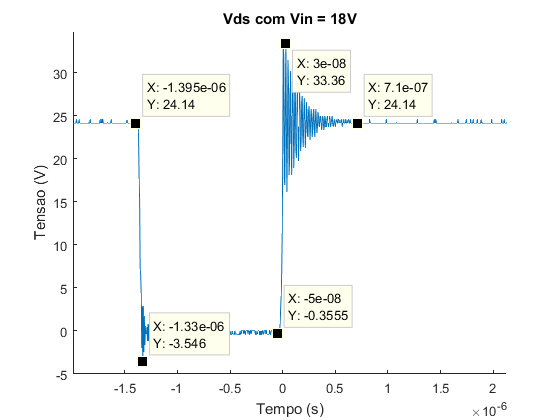
\includegraphics[width=0.8\textwidth]{vds-18V.png}
	\caption{Tensão dreno-fonte para @Vin=18V.}
	\label{fig:vds-18V}
\end{figure}

\begin{figure}[H]
	\centering
	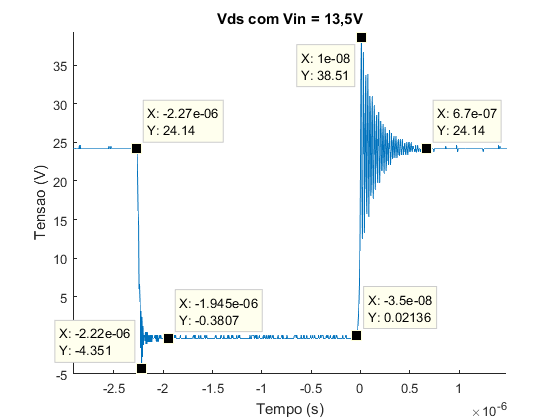
\includegraphics[width=0.8\textwidth]{vds-13V5.png}
	\caption{Tensão dreno-fonte para @Vin=13V5.}
	\label{fig:vds-13V5}
\end{figure}

\begin{figure}[H]
	\centering
	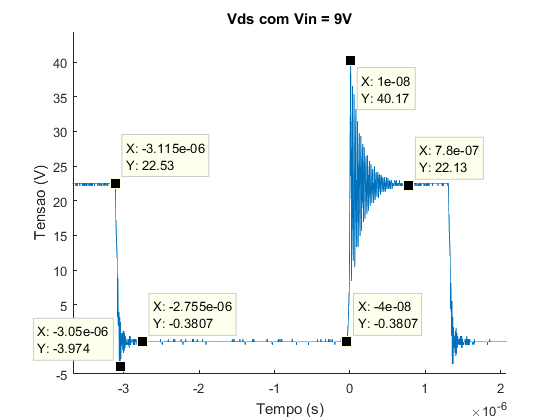
\includegraphics[width=0.8\textwidth]{vds-9V.png}
	\caption{Tensão dreno-fonte para @Vin=9V.}
	\label{fig:vds-9V}
\end{figure}


\clearpage

\section{Conclusões}
\label{sec:conclusoes}

Como se pôde notar na Seção \ref{sec:resultados}, o conversor \emph{Boost} não atendeu todas as especificações de projeto. Um indicativo de que havia algo errado foi o fato do indutor estar aquecendo consideravelmente. Ao percebê-lo, reviram-se os cálculos e notou-se que as correntes eficaz e de pico levadas em conta nas Equações \ref{eq:b-max-erro} e \ref{eq:area-erro} estão mal levantadas. O correto seria ter considerado os valores de pico da simulação (Seções \ref{subsub:corrente-media} e \ref{subsub:corrente-max}). Com o indutor aquecendo, o material do carretel, produzido em impressora 3D, começou a amolecer. Isso causou a diminuição do entreferro (devido ao peso do núcleo estar sobre o carretel), levando à saturação. Com o núcleo saturado, o indutor não conseguia fornecer a corrente necessária para suprir a demanda. Com isso, percebe-se que, nos casos em que há maior demanda de corrente (por exemplo, Figura \ref{fig:ripple-9V}), a tensão de saída fica muito abaixo dos 24V esperados.

Observou-se também que a simulação apresentou valores não condizentes com o caso real. Como pode-se notar na Seção \ref{subsub:vds}, os valores das tensões entre dreno e fonte foram maiores que os apresentados na
Seção \ref{subitem:vds}. Por sorte, os valores reais estavam dentro do limite suportado pelo \emph{Mosfet}.

% A plataforma foi construída em uma estrutura de madeira, contendo uma base e uma coluna. O mecanismo desenvolvido para permitir a inclinação é bastante simples, apresentando dois pontos fixos e uma articulação que acompanha a inclinação da plataforma. É composto ainda, por duas peças que funcionam como uma haste de amortecedor. Uma das peças é fixa na base e outra é articulada na plataforma. Nos parafusos de fixação destas peças, é presa uma mola responsável por fazer com que o mecanismo retorne à sua posição inicial.
% Na Figura \ref{fig1} os componentes do sistema são apresentados, onde:
% \begin{itemize}
% \item \hspace{2mm} 1 -- Base da estrutura;
% \item \hspace{2mm} 2 -- Plataforma;
% \item \hspace{2mm} 3 -- Centro de giro da plataforma;
% \item \hspace{2mm} 4 --  Coluna;
% \item \hspace{2mm} 5 -- Ponto de articulação;
% \item \hspace{2mm} 6 -- Anteparo de alumínio;
% \item \hspace{2mm} 7 -- Sensor de ultrassom;
% \item \hspace{2mm} 8 -- Ponto de fixação à base.
% \end{itemize}
%   \begin{figure}[H]
%     \centering
%     \includegraphics[height=7cm]{Detalhamento}
%     \caption{Componentes do sistema.}
%     \label{fig1}
%   \end{figure}

% O sensor de ultrassom é posicionado em um suporte na peça fixa à base, a uma distância de 70mm do ponto de fixação, de forma a medir a distância até uma chapa de alumínio, fixada na peça articulada a uma distância 25mm do ponto de articulação.
% Na plataforma, uma chapa de aço de pequena dimensão foi centrada a fim de manter um medidor de ângulo com base magnética. A Figura \ref{fig2a}, apresenta o CAD da estrutura, enquanto em \ref{fig2b} é possível observar o resultado da construção.

% \begin{figure}[H]
% \centering
% \subfloat[CAD da estrutura da plataforma.]{
% \includegraphics[height=7cm]{Montagem_trimetric}
% \label{fig2a}
% }
% \quad %espaco separador
% \subfloat[Estrutura finalizada.]{
% \includegraphics[height=7cm]{View3}
% \label{fig2b}
% }
% \caption{Estrutura construída para medição de ângulo de inclinação da plataforma.}
% \label{fig2}
% \end{figure}

% \subsection{Modelo Matemático do Mecanismo}
% O mecanismo adotado para a conversão de um movimento linear em angular é baseado em uma soma de vetores, condição de viabilidade do mecanismo. A Figura \ref{fig3} apresenta o diagrama analisado.
%   \begin{figure}[H]
%     \centering
%     \includegraphics[height=7cm]{Dimens_o}
%     \caption{Diagrama do mecanismo utilizado.}
%     \label{fig3}
%   \end{figure}
% A partir do diagrama, é realizada a soma vetorial das componentes em x e em y, ou seja, $\sum _{x}=0$ e $\sum _{y}=0$, conforme as equações \ref{eq1} e \ref{eq2} abaixo.

% \begin{equation}
% L_{2}cos(\beta) - L_{1}cos(\alpha) + X_{1} = 0 
% \label{eq1}
% \end{equation}

% \begin{equation}
% L_{2}sen(\beta) - L_{1}sen(\alpha) + Y_{1} = 0
% \label{eq2}
% \end{equation}

% Como a variável de interesse é a distância que deverá ser medida pelo sensor, isto é, a distância entre a chapa de alumínio utilizada como anteparo e o sensor há ainda a relação da equação \ref{eq3}:

% \begin{equation}
% -L_{3} - T_{1} - T_{2} + L_{2} = 0
% \label{eq3}
% \end{equation}

% Onde
% \begin{itemize}
% \item \hspace{2mm} $L_{1} $ -- Distância entre o centro de giro da plataforma e o centro de articulação;
% \item \hspace{2mm} $L_{2} $ -- Distância entre o ponto de articulação e o ponto de fixação da haste à base;
% \item \hspace{2mm} $L_{3} $ -- Distância entre a chapa de alumínio e o sensor de ultrassom;
% \item \hspace{2mm} $Y_{1} $ -- Distância vertical entre o centro de giro da plataforma e o ponto fixo à base;
% \item \hspace{2mm} $X_{1} $ -- Distância horizontal entre o centro de giro da plataforma e o ponto fixo à base;
% \item \hspace{2mm} $T_{1}$ -- Distância entre o ponto de articulação e a chapa de alumínio;
% \item \hspace{2mm} $T_{2}$ -- Distância entre o sensor e o ponto fixo à base;
% \item \hspace{2mm} $\alpha$ -- Ângulo de inclinação da plataforma;
% \item \hspace{2mm} $\beta$ -- Ângulo de inclinação das hastes.
% \end{itemize}

% A análise da estrutura construída é necessária para determinar se a relação do ângulo de inclinação e o deslocamento axial das hastes possui comportamento linear e então, determinar e aplicar as equações de calibração do sinal de resposta do sensor. Assim, um script em \textit{Matlab} aplica o Método de Newton-Raphson a partir de chutes iniciais que correspondem à inclinação de $0^\circ$ da plataforma. O modelo converge e como resultado, apresenta valores dos ângulos $\alpha$ e $\beta$. O ângulo de interesse ($\alpha$) em função de $L_{2}$ tem comportamento muito próximo da linearidade para ângulos até $50^\circ$ (Figura \ref{fig4}).
%   \begin{figure}[H]
%     \centering
%     \includegraphics[width=14cm]{Resposta.png}
%     \caption{Resposta do método matemático para o sistema.}
%     \label{fig4}
%   \end{figure} 
% Por regressão linear, a equação \ref{eq4} apresenta a relação a função que relaciona o ângulo de inclinação $\alpha$ e o deslocamento da haste como variação do comprimento $L_{2}$.
% \begin{equation}
% \alpha=0,32496 L_{2} - 84,18
% \label{eq4}
% \end{equation}

% \section{Aquisição de Dados}

% Para a aquisição de dados, foi utilizado o kit \textit{LaunchPad Tiva C Series TM4C123G}, da \textit{Texas Instruments}, contendo o microcontrolador ARM Cortex-M4F de 32 bits, operando em 80MHz, o que proporciona melhor resolução dos dados aquisitados. Os dados foram mostrados na serial em intervalos de 0,25 segundos.

% O funcionamento do sensor HC-SR04 é baseado em reflexão de ondas sonoras ao atingir algum objeto. Um sinal nível alto de $10\mu s$ deve ser colocado no pino de trigger para que se inicie a medição. O módulo então, envia 8 pulsos de 40kHz e quando o sinal for refletido por um objeto e detectado pelo receptor, o pulso de saída no pino echo passa do nível lógico alto para baixo. Portanto, tem-se uma duração do pulso, que significa quanto tempo decorreu desde o envio do sinal até seu retorno.

% Para realizar a aquisição dos dados, o pino echo do sensor foi ligado à porta PB1 do \textit{Tiva}, configurada como entrada digital. O pino de trigger recebe o pulso da saída digital PB0. O esquemático da Figura \ref{fig5} mostra as conexões entre o módulo e a placa.
% \begin{figure}[H]
%     \centering
%    \includegraphics[width=9cm]{Esquematicoet1.png}
%     \caption{Esquemático das conexões realizadas.}
%     \label{fig5}
%   \end{figure}
  
%   Vale ressaltar que o \textit{Tiva} suporta apenas tensões de no máximo 3,6V, enquanto o módulo apresenta um nível alto em 5V. Por esse motivo, um resistor de $1k\Omega$ foi empregado para abaixar o nível de tensão na entrada e evitando a danificação/queima da porta. A alimentação do HC-SR04 deve ser 5V e por esse motivo, foi utilizado o pino VBUS do \textit{Tiva} para alimentação do mesmo. O microcontrolador foi programado em C, utilizando o compilador \textit{Code Composer Studio}.
  
% \subsection{Método Experimental}
% Para validar o modelo matemático, medidas foram realizadas na estrutura construída. Com a ajuda de um medidor de ângulo, o ângulo foi submetido à variações de $0^\circ$ a $50^\circ$ de inclinação em passos de $5^\circ$. No gráfico da Figura \ref{fig6}, pode ser observada a curva obtida com as medidas do sensor.
% \begin{figure}[H]
%     \centering
%    \includegraphics[width=14cm]{Medidas}
%     \caption{Resposta das medições experimentais.}
%     \label{fig6}
%   \end{figure}
%   Por regressão linear determinou-se a equação que rege o comportamento do ângulo em função da variação do comprimento $L_{3}$, distância entre o sensor e o anteparo, observada na equação \ref{eq5}.
% \begin{equation}
% \alpha=0,33238 L_{2} - 61,496
% \label{eq5}
% \end{equation}

% A diferença identificada entre os coeficientes do modelo matemático e prático, em especial o coeficiente linear, se deu principalmente pelas não idealidades na etapa de construção, pois as maiores fontes de erro são nas distâncias dos ponto de giro da plataforma e dos pontos de fixação, que apresentaram diferenças na ordem de centímetros. A Figura \ref{fig7} mostra a montagem para a realização do ensaio.

% \begin{figure}[H]
%     \centering
%     \includegraphics[width=12cm]{View4}
%     \caption{Montagem para a realização de medições experimentais.}
%     \label{fig7}
%   \end{figure}

% \subsection{Calibração}
% Conhecendo o funcionamento do sensor em questão, pode-se afirmar que são necessárias duas etapas de calibração. A primeira delas é transformar a duração do pulso lido na porta de entrada digital do Tiva proveniente do pino echo do sensor. Essa transformação fornece um valor de distância que o sensor mediu até o anteparo ou objeto. Essa primeira equação está apresentada em \ref{eq6}, onde d é a distância medida e T é a duração do pulso.
% %FALTA EXPLICAR O PROGRAMA NO CCS COM A LÓGICA DE TIMER PARA CALCULAR A DURAÇÃO.
% \begin{equation}
% d= \left( \frac{340T}{2} \right) 100
% \label{eq6}
% \end{equation}

% A segunda etapa de calibração é a aplicação da equação encontrada pelas medidas experimentais no sistema físico construído. A relação está expressa na equação \ref{eq5}, explicitada na seção anterior. Dessa forma, a duração do pulso medida é transformada em uma distância e então, em um ângulo, que será utilizado na próxima etapa do projeto para a atuação sobre um motor.
% As medidas realizadas com o sensor para os principais ângulos, estão apresentadas na Tabela \ref{t1}.
% \begin{table}[h]
% \centering
% \caption{Medidas realizadas com o sinal calibrado.}
% \begin{tabular}{c|c}
% Ângulo de Inclinação $\alpha$ & Distância Medida [cm] \\ 
% \hline                           $0^\circ$     &  19,19    \\
% $5^\circ$     &		19,91	\\
% $10^\circ$     &        22,43 \\
% $15^\circ$      &   23,76\\
% $20^\circ$       &    25,4\\
% $25^\circ$     &27,1\\
% $30^\circ$      &   28,59     \\
% $35^\circ$       &   30,12\\
% $40^\circ$        &   31,66\\
% $45^\circ$    &33,05\\
% $50^\circ$     & 33,92           
% \end{tabular}
% \label{t1}
% \end{table}
% \section{Atuação}
% Na etapa de atuação, a conversão digital-analógica por PWM (\textit{Pulse Width Modulation}) foi utilizada para o acionamento e controle de velocidade do motor DC. Com PWM de 8 bits, é possível garantir uma resolução adequada a fim de evitar instabilidade do atuador. A frequência configurada do PWM foi de 4,9kHz.
% \subsection{Circuito de Atuação}
% Para o acionamento do motor DC por PWM, foi necessário o projeto de um circuito de chaveamento que respondesse à saída PWM do pino PB7 do microcontrolador. O circuito é composto por um transistor de potência MOSFET canal tipo N, CSD18502KCS, o diodo de proteção e capacitores para filtragem da alimentação. Para a determinação do transistor a ser utilizado, foi medida a corrente do atuador, um motor DC de 12V. A corrente medida de 1,46A permite o cálculo da resistência elétrica do motor, e portanto pela Lei de Ohm (\ref{eq7}):
% \begin{equation}
% R_{motor}=\frac{V}{I}=\frac{12}{1,46}=8,219 \Omega
% \label{eq7}
% \end{equation}

% Além da corrente da carga, outro importante fator para a escolha do transistor utilizado no circuito de chaveamento é a resistência entre dreno e fonte $R_{DS}$.
% Para que não haja considerável queda de tensão entre os terminais de dreno e fonte, e consequentemente maior perda de energia por efeito Joule no transistor (dissipação de potência devido ao aquecimento, a resistência $R_{DS}$ deve ser menor que $1\%$ da resistência da carga, no caso, o motor. Utilizando a equação \ref{eq8}, pode-se aproximar o valor de $R_{DS}$. Para o transistor CSD18502KCS (Anexo C), para as condições de operação desta aplicação, tem $R_{DS}$ aproximado:
% \begin{equation}
% R_{DS}=\dfrac{1}{2 g_{m}(V_{GS}-V_{TH})}=\dfrac{1}{2*138 (3,3-2,1)}=3,019m\Omega
% \label{eq8}
% \end{equation}

% O valor de transcondutância $g_{m}$, bem como o valor da tensão de limiar $V_{TH}$, foram obtidos na folha de dados do componente. O cálculo de $R_{DS}$ é necessário pois não são fornecidas informações suficientes para um valor de $V_{GS}$ igual a 3,3V, tensão em nível alto de saída do Tiva. O $g_{m}$ indicado na folha de dados é de 138, enquanto o valor da tensão máxima $V_{TH}$ (Tensão de Threshold) é de 2,1V (valor típico 1,8 V). Esse valor indica que o transistor precisa superar a queda de 2,1V entre os terminais porta e fonte a fim de chavear. Isso significa que, aplicando uma tensão de 3,3 V na porta, é possível fazer com que o transistor passe a conduzir. Considerando o pior caso ($V_{TH}$ máximo de 2,1V), como resultado da aplicação da equação \ref{eq8} obtém-se a resistência aproximada $R_{DS} =$3,019m$\Omega$ e que corresponde a 0,036$\%$ da resistência do motor. O esquemático do circuito de chaveamento é apresentado na Figura \ref{fig8}.
% \FloatBarrier
% \begin{figure}[H]
%     \centering
%     \includegraphics[width=14cm]{Esquematico}
%     \caption{Esquemático do circuito de atuação.}
%     \label{fig8}
% \end{figure}
% \FloatBarrier

% A montagem de circuitos em matrizes de contatos são adequadas apenas para montagens experimentais. Além de baixa capacidade de corrente, a capacitância e resistência dos contatos internos são consideráveis e são suscetíveis à captação de ruídos e interferências externas indesejáveis. Para esta etapa do projeto, uma placa de circuito impresso foi projetada (Figura \ref{fig9}), por se tratar de um circuito de chaveamento e com circulação de correntes relativamente elevadas, onde o motor drena da fonte acima de 1,4A. Para o projeto da placa de circuito impresso foi utilizado o \textit{software Altium Designer}.

% \begin{figure}[H]
% \centering
% \subfloat[2D.]{
% \includegraphics[height=5cm]{Placa_2D}
% \label{fig9a}
% }
% \quad %espaco separador
% \subfloat[3D.]{
% \includegraphics[height=5cm]{Placa_3D_01}
% \label{fig9b}
% }
% \caption{Projeto da placa de circuito impresso.}
% \label{fig9}
% \end{figure}
% \FloatBarrier

% Como o circuito de chaveamento demanda corrente elevada, provoca a propagação de variações na tensão de alimentação para o restante do circuito. Este efeito foi minimizado pelo uso de capacitores de desacoplamento ligados em paralelo e muito próximos da alimentação do circuito de chaveamento. Cada um destes capacitores é responsável por suprir rápidos transientes de corrente sem que ocorra variação na alimentação. Foram usados os valores de $100 \mu F$, $100nF$ e $10nF$.


% \section{Análise Estatística dos Dados do Sensor}
% A avaliação de relação sinal-ruído é um importante parâmetro para a avaliar o desempenho do sistema. O significado físico do SNR é quantas vezes o sinal é maior do que o ruído inerente a interferências externas no sistema.
% A fim de avaliar o valor do SNR do sistema, foi realizada uma aquisição de 150 pontos, com frequência de amostragem igual a 120Hz. O cálculo do SNR foi possível através da equação \ref{eq9}. Para a aquisição, o ciclo de trabalho do PWM foi setado para 50\% e a rampa fixada com um ângulo de inclinação de aproximadamente 25$^{\circ}$.

% \begin{equation}
% SNR=\frac{\overline x}{\sigma _{x}}
% \label{eq9}
% \end{equation}

% Onde
% \begin{itemize}
% \item \hspace{2mm} $\overline x$ -- média dos pontos aquisitados;
% \item \hspace{2mm} $\sigma _{x}$ -- desvio padrão.
% \end{itemize}

% Portanto, o SNR calculado para média obtida igual a 24,9915$^{\circ}$, enquanto o desvio padrão foi de 0,0143, o que resulta em um SNR$=$1747,416. A Figura \ref{fig10} apresenta um gráfico das medidas realizadas para ângulo fixo aproximado de $25^o$ em função do número da amostra, possibilitando a visualização da variação nas medidas com as quais o SNR foi calculado.  

% Inicialmente, o código implementado foi escrito e compilado na ferramenta Code Composer Studio, utilizando uma biblioteca de auxilio ao desenvolvimento dedicada a este microcontrolador conhecida como TivaWare (Anexo A). Porém as medições da relação sinal-ruído com a aplicação deste código não atingiram o valor mínimo esperado de 100. Os valores de SNR variavam de 30 a 80 aproximadamente. O problema da baixa SNR esta diretamente relacionada ao controle do sistema, pois um valor de medição que varia muito pode causar oscilações em torno do valor final esperado. Devido a incerteza da origem do problema que poderia causar estas oscilações e já tendo tomado as devidas precauções em relação a hardware, optou-se então por alterar o ambiente de desenvolvimento do código. A segunda opção foi o Energia, o que permite programar o microcontrolador usando uma linguagem mais simples, muito parecida com a do Arduino (Anexo B). A medida da SNR com este novo código melhorou mas não de forma significativa. Como uma nova forma de melhora da SNR, agora a nível de software, um filtro digital conhecido como média móvel foi aplicado ao sistema de medição. O valor final da medição é igual a média de um número de medições anteriores e isso tem como efeito a diminuição da variação dos valores medidos, porém isto leva também a um aumento da ordem do sistema, mais um zero, o que dificulta o processo de controle.  

% \begin{figure}[H]
%     \centering
%     \includegraphics[width=16cm]{41.png}
%     \caption{Gráfico das Medidas Realizadas para Calculo do SNR.}
%     \label{fig10}
%   \end{figure}

% \section{Identificação do Sistema}

% \subsection{Análise da Resposta Temporal do Conjunto Sensor/Atuador}

% Utilizando uma frequência de amostragem de 20Hz (taxa de amostragem igual a 50ms), foram obtidos 155 pontos medidos durante o tempo de transição da resposta do sensor com a aplicação de um degrau de 150 a 200 no valor do PWM. Esse degrau foi escolhido, de forma a iniciar as medidas com o motor já em movimento, o que evito erros de amostragem devido ao atrito estático e a inércia associada a operação do motor DC. Os dados obtidos são apresentados no gráfico da Figura \ref{fig11}, com as medidas em função do tempo. Outro fator relevante é que os dados de PWM também foram aquisitados, permitindo conhecer o instante exato da aplicação do degrau. A resposta temporal resultante do ensaio para a aquisição dos dados, apresenta um comportamento de segunda ordem subamortecido devido a aplicação da média móvel. Porém, esse comportamento deverá ser validado pela função de transferência.

% \begin{figure}[H]
%     \centering
%     \includegraphics[width=16cm]{24.png}
%     \caption{Resposta Temporal do Sistema com Aplicação de Degrau no PWM.}
%     \label{fig11}
%   \end{figure}

% \subsection{Obtenção do Modelo Matemático}

% Com os dados obtidos, o \textit{Matlab} foi usado para encontrar o modelo matemático que melhor se aproxima do comportamento dinâmico do sistema, utilizando a ferramenta \textit{System Identification}. As variáveis de entrada e saída foram importadas para o ambiente de análise e o tempo de amostragem configurado para 50 milisegundos. A estimativa é realizada na opção \textit{Process Models}, onde foram determinados parâmetros como número de pólos e zeros (2 e 0, respectivamente). O \textit{default} dessa ferramenta é considerar um atraso até a aplicação do degrau, o que implica na adição de um termo exponencial na função de transferência. Como os dados foram normalizados, o atraso não é considerado.
% Como resultado, foram retornados os valores de k, Tw, e Zeta $(\zeta)$ resultando a função transferência da equação \ref{eq2h}. A resposta normalizada pode ser observada na Figura \ref{fig11}.

% \begin{equation}
% PV(s)=k \dfrac{\omega _{n}^2}{s^2 + 2 \zeta \omega _{n} s + \omega _{n}^2}=\dfrac{k}{1 + (2 \zeta Tw)s +Tw^2s^2}
% \label{eq23}
% \end{equation}

% Onde:
% \begin{itemize}
% \item \hspace{2mm} k é o ganho do sistema;
% \item \hspace{2mm} Tw é o inverso da frequência natural $\omega _{n}$ de oscilação (sem amortecimento);
% \item \hspace{2mm} $\zeta$ é o fator de amortecimento. 
% \end{itemize}

% \begin{equation}
% PV(s)= \dfrac{0,17384}{1+0,8814s+0,2825s^2}
% \label{eq2h}
% \end{equation}.

% \begin{figure}[H]
%     \centering
%    \includegraphics[width=17cm]{25.png}
%     \caption{Resposta Normalizada do Sistema.}
%     \label{fig11}
%   \end{figure}
% \FloatBarrier
% A ferramenta \textit{System Identification} retorna o ajuste da função transferência estimada, com os dados da aquisição. O nível, em porcentagem, de coincidência foi igual a $95,76\%$. Esse resultado pode ser observado na Figura \ref{fig12}.

% \begin{figure}[H]
%     \centering
%    \includegraphics[width=17cm]{26.png}
%     \caption{Função Transferência Estimada pelo \textit{System Identification}.}
%     \label{fig12}
%   \end{figure}
% \FloatBarrier

% \subsubsection{Análise Comparativa}
% Comparando as duas funções encontradas, a fim de determinar a melhor aproximação com a medida realizada no ensaio, a ferramenta \textit{Simulink} foi utilizada com o esquemático da Figura \ref{fig13}. 
% \begin{figure}[H]
%     \centering
%     \includegraphics[width=9cm]{22.png}
%     \caption{Função Transferência Utilizada no \textit{Simulink}.}
%     \label{fig13}
%   \end{figure}
  
% Na simulação, o Step foi configurado com valor inicial igual a 0 e final 50. A Figura \ref{fig15} mostra a comparação entre a estimativa via \textit{software} e compara o modelo (Figura \ref{fig14}) com as medidas realizadas.

% \begin{figure}[H]
%     \centering
%     \includegraphics[width=17cm]{27.png}
%     \caption{Resposta ao Degrau da Função Transferência Estimada.}
%     \label{fig14}
%   \end{figure}

% Nota-se que a estimativa obtida pelo \textit{System Identification} ficou muito próxima da resposta do sistema, de forma que representou de forma adequada o comportamento do conjunto sensor mais atuador.
% \begin{figure}[!ht]
%     \centering
%    \includegraphics[width=17cm]{40.png}
%     \caption{Comparação entre Dados de Aquisição e Função Transferência.}
%     \label{fig15}
%   \end{figure}


% \section{Controlador PID}
% \subsection{Determinação dos Parâmetros do Controlador}

% \subsubsection{Método Ziegler Nickols}
% O método de Ziegler Nickols está baseado na resposta ao degrau do sistema em malha aberta. Com a resposta ao degrau de 0 a 8 segundos, tem-se, na Figura \ref{fig17}:
% \begin{figure}[!ht]
%   \centering
%   \includegraphics[width=16.4cm]{29.png}
%     \caption{Determinação dos parâmetros do controlador.}
%     \label{fig17}
%   \end{figure}
% \FloatBarrier
% Como apresenta o gráfico, foram traçadas dois segmentos de reta, um delas sendo a reta tangente que passa pelo ponto de inflexão durante a subida. Outra reta corresponde a constante k de ganho do sistema e igual a razão entre o valor em regime permanente e o degrau aplicado, como na Equação.
% \begin{equation}
% k = \dfrac{8,69}{50} = 0,1738
% \end{equation}

% O valor L corresponde ao intervalo de tempo até que a reta tangente cruze o eixo do tempo, assumindo o valor de 0,5 segundos. Desse instante até o instante de tempo em que a reta tangente cruza a reta do valor de k, denomina-se o valor de T e equivale a 1,19 segundos. Com o tempo de amostragem $T_{s}$ igual a 50 milisegundos, calcula-se as constantes do controlador PID: $K_{p}$, $K_{i}$ e $K_{d}$	
% \begin{equation}
% K_{p}=\dfrac{1,2}{k}\dfrac{T}{L}=\dfrac{1,2}{0,1738}\dfrac{1,19}{0,5}=16,435
% \end{equation}
% \begin{equation}
% K_{i}=\dfrac{0,6}{k}\dfrac{T}{L^2}T_{s} =K_{p}\dfrac{T_{s}}{2L}=0,8215
% \end{equation}
% \begin{equation}
% K_{d}=\dfrac{1,2}{k}\dfrac{T}{T_{s}}=K_{p}\dfrac{L}{T_{s}}=164,35
% \end{equation}

% \subsubsection{Método PID Tuner - Matlab}
% Uma das formas de projetar o controlador PID de um sistema é através do software \textit{Matlab} usando a opção PID Tuner. O projeto do controlador tem como base a planta do sistema e entrando com os dados de aquisição normalizados em resposta ao degrau, ajustando o sinal de entrada e tempo de amostragem a ferramenta calcula automaticamente a planta. Como a primeira identificação do sistema havia sido feita no MATLAB, o resultado do processo acima descrito foi muito parecido com o já obtido anteriormente.
% O controlador escolhido foi do tipo PID e os parâmetros da resposta normalizada que ficam acessíveis ao usuário como tempo de resposta e comportamento transitório foram fixados em 0,8387 e 0,74, respectivamente. Como resultado, o valor das constantes do controlador PID: 
% $K_{p}$, $K_{i}$ e $K_{d}$ foram as seguintes: $K_{p}=1,484$, $K_{i}=1,637$ e $K_{d}=2,857$.

% O gráfico da Figura \ref{fig18} abaixo representa a resposta normalizada do sistema em malha fechada após atuação do controlador.

% \begin{figure}[!ht]
%   \centering
%   \includegraphics[height=8.8cm]{30.png}
%     \caption{Resposta sistema com controlador em malha fechada.}
%     \label{fig18}
%   \end{figure}
% \FloatBarrier


% \subsection{Análise Temporal do Sistema Realimentado}

% A implementação do controlador PID a nível digital, foi inicialmente feita com as constantes encontradas pelo método Ziegler Nickols. No entanto, o comportamento do sistema se mostrou instável, com oscilação em torno do \textit{setpoint} de aproximadamente $10^o$. A Figura \ref{fig19} apresenta a resposta do sistema em malha fechada. Para a obtenção dessa resposta, a plataforma se encontrava com inclinação $0^o$ devendo atingir aproximadamente $30\%$ do ângulo máximo de $45^o$. 

% \begin{figure}[!ht]
%   \centering
%   \includegraphics[width=17cm]{44.png}
%     \caption{Resposta do Sistema para Inclinação de $13^o$.}
%     \label{fig19}
%   \end{figure}
% \FloatBarrier

% A resposta também foi analisada para a inclinação inicial aproximada de $0^o$ com \textit{setpoint} igual a $30^o$ que corresponde a aproximadamente $70\%$ do ângulo de inclinação máximo, como pode ser observado na Figura \ref{fig20}. De mesma forma, a resposta apresenta variações de aproximadamente $7^o$ em torno do \textit{setpoint}.

% \begin{figure}[!ht]
%   \centering
%   \includegraphics[width=17cm]{46.png}
%     \caption{Resposta do Sistema para a Inclinação de $30^o$.}
%     \label{fig20}
%   \end{figure}
% \FloatBarrier
% Buscando solucionar o problema e Utilizando a ferramenta \textit{PID Tuner}, há a possibilidade de ajustar robustez e velocidade de resposta, de forma que foram obtidos diferentes para as constantes. No entanto, com os valores já explicitados na subseção anterior, o valor do erro em regime permanente estava acima da especificação e, portanto, optou-se por ajustar manualmente nos valores resultantes, tendo como prioridade o aumento da constante proporcional, depois constante integrativa e por último da constante derivativa. 

% Sabendo que o tempo de resposta pode ser ajustado de acordo com o valor da constante $K_{p}$, premissa da determinação das constantes do controlador pela ferramenta \textit{PID Tuner}, foram feitas alterações no valor dessa constante de forma a permitir uma resposta mais rápida, ou seja, possibilitando atingir o valor desejado de \textit{setpoint} no menor tempo possível e respeitando as especificações mínimas de desempenho. Aumentando a constante $K_{p}$, foi observado maior erro em regime permanente, que violava a condição de erro inferior a $2\%$. Por esse motivo, foi também necessário aumentar o valor da constante $K_{i}$ para que o erro em regime permanente pudesse atender à condição imposta. Como consequência, a sobrelevação da resposta no transitório passou a ser mais significativa, fazendo com que o valor da constante $K_{d}$ também fosse incrementado. 

% A Figura \ref{fig21} apresenta o resultado para a inclinação de $15^o$, aproximadamente $30\%$ da inclinação máxima da plataforma. Com o \textit{setpoint} de $15^o$, o valor da inclinação em regime permanente foi igual a $15.07^o$, ou seja, o erro foi próximo a $0,15\%$ apenas, além de não apresentar sobrelevação e alcançar o valor desejado em aproximadamente 15 segundos.

% \begin{figure}[!ht]
%   \centering
%   \includegraphics[width=17cm]{34.png}
%     \caption{Resposta do Sistema para a Inclinação de $15^o$.}
%     \label{fig21}
%   \end{figure}
% \FloatBarrier

%  De mesma forma, a resposta foi analisada para a inclinação de $30^o$, apresentada na Figura \ref{fig22}.

% \begin{figure}[!ht]
%   \centering
%   \includegraphics[width=17cm]{36.png}
%     \caption{Resposta do Sistema para a Inclinação Inclinação de $30^o$.}
%     \label{fig22}
%   \end{figure}
% \FloatBarrier

%  Com inclinação inicial de $0^o$, o valor desejado de inclinação foi alcançado em 20 segundos. O valor em regime permanente foi igual a $29.69^o$, o que gera um erro de aproximadamente $0,7\%$. A sobrelevação observada na resposta também atende às especificações de forma que o valor máximo de $31,42^o$ representa $3,15\%$.
% Para que fossem obtidos esses resultados, como sendo os resultados que melhor se enquadram nas especificações de desempenho, os valores das constantes do controlador utilizadas foram $K_{p}=1$, $K_{i}=0,1$ e $K_{d}=6$.





% \newpage
% \section*{Conclusões}
% \addcontentsline{toc}{section}{\protect\numberline{}Conclusões}%

% Durante o desenvolvimento das quatro etapas do projeto puderam ser compreendidas as particularidades da implementação de um sistema de controle. Podem ser destacadas portanto, as conclusões em cada uma das etapas até o efetivo controle de inclinação de uma plataforma plana.

% Na primeira etapa, os maiores desafios corresponderam à concepção de uma estrutura mecânica através da qual fosse possível relacionar a leitura de um sensor de ultrassom com a inclinação da plataforma que compõe a estrutura. A modelagem matemática da estrutura se mostrou de grande importância nas etapas posteriores, pois determina a equação de calibração implementada a nível de \textit{software} e que possibilitou a leitura com certa precisão da grandeza que se desejava medir: a inclinação em graus da plataforma.

% A partir da leitura dos dados, o projeto de um circuito de atuação leva em consideração os efeitos no sistema como um todo, levando à análise do comportamento dos componentes do circuito, interferências externas, eletromagnéticas e também a influência da indutância dos cabos de conexão com a alimentação. Entre outras influências, pode ser citada a grande diferença identificada na relação sinal-ruído causada pela vibração mecânica em consequência do desbalanceamento da hélice acoplada ao eixo do motor. Ainda que o projeto do circuito de atuação fosse projetado com capacitores de desacoplamento próximos ao transistor de chaveamento, dimensão reduzida de cabos, a vibração mecânica se mostrou determinante no desempenho do sistema. O aumento na relação sinal-ruído após o balanceamento da hélice e a utilização de um fonte estabilizadora foi considerável. As não idealidades do sistema foram corrigidas com a implementação da médida móvel, que resultou em uma SNR superior a 100 vezes da SNR obtida inicialmente, destacando a eficácia de diversas técnicas para o aumento da relação-ruído em um sistema.

% Durante a etapa de identificação mecânica, também foi observada falta de coerência entre a qualidade dos dados de aquisição com a aplicação de um degrau no PWM e SNR. A montagem da hélice feita de maneira equivocada resultou em perda de eficiência com relação ao empuxo gerado e por esse motivo, o sistema apresentava uma resposta muito lenta e que causava oscilações na leitura do sensor de ultrassom. A solução não se encontrava, portanto, em quaisquer alterações de \textit{software} mas, novamente, de \textit{hardware}. A importância da construção na primeira etapa ficou evidente, de forma que todas as demais etapas foram comprometidas, de certa forma, por questões de construção como atrito, desequilíbrio com o centro de giro, desbalanceamento da hélice.

% A implementação do controle de um controlador PID em \textit{software} se mostrou bastante simples. No entanto, esse resultado somente foi alcançado devido a leitura correta do ângulo de inclinação a partir do sensor de ultrassom, contando com uma SNR que permitiu alta qualidade dos dados amostrados, proporcionando a correta identificação do sistema. O valor das constantes do controlador, proporcional, intergral e derivativo, quando calculadas usando o método do Ziegler Nickols e aplicadas ao controle tiveram como efeito uma resposta instável e com oscilação extremamente grande. Respeitando os limites de \textit{overshoot} e erro em regime permanente, as constantes calculadas pelo método anterior não se mostraram adequadas. Assim, com os novos valores calculados para as constantes através do método \textit{PID Tuner} disponível no \textit{Matlab}, foi possível se aproximar de uma resposta ótima e a ferramenta se mostrou interessante devido a possibilidade de ajuste de robustez e velocidade de resposta esperada. Por fim, ajustes empíricos necessários foram justificados pela melhora significativa da resposta e confirmou-se a necessidade de experimentação e compreensão do método e do significado das constantes do controlador e qual a função que cada uma desempenha para que o controle seja efetivo.

% O projeto como um todo pode elucidar dúvidas a respeito da implementação e do objetivo prático de sistemas de controle, desde a fundamental etapa de condicionamento de sinal de sensores e calibração. Permitiu, portanto, o conhecimento prático de problemas que envolvem variáveis sobre as quais se tem controle, mas também sobre outras cujas causas são desconhecidas, caracterizando erros aleatórios que puderam ser minimizados através de técnicas aprendidas na disciplina de Instrumentação Eletrônica.

% \newpage
% \section*{Referências Bibliográficas}
% \addcontentsline{toc}{section}{\protect\numberline{}Referências Bibliográficas}%

% \noindent [1] PULSE WIDTH MODULATION -- DC MOTOR DRIVES -- ELECTRONICS TEXTBOOK
% "Pulse Width Modulation | DC Motor Drives | Electronics Textbook", Allaboutcircuits.com, 2017. [Online]. Disponível em:
% https://www.allaboutcircuits.com/textbook/semiconductors/ chpt-11/pulse-width-modulation/
% \\

% \noindent [2] COMO UTILIZAR O SENSOR ULTRASÔNICO HC-SR04
% "Como utilizar o sensor ultrasônico HC-SR04", Buildbot.com.br, 2017. [Online]. Disponível em: http://buildbot.com.br /blog/como-utilizar-o-sensor-ultrasonico-hc-sr04/
% \\

% \noindent [3] GUIDE\_TM4C123LAUNCHPAD
% "Guide\_TM4C123LaunchPad", Energia.nu, 2017. [Online]. Disponível em: http://energia.nu/pin-maps/guide\_tm4c123launchpad/
% \\

% \noindent [4] PROJETOS - CÁLCULOS
% "Projetos - Cálculos", Diydrones.com, 2017. [Online]. Disponível em: http://diydrones.com/group/brazilian-group-drone/forum/topics/projetos-c-lculos.
% \\

% \noindent [5] PID CONTROLLER TUNING BASED ON MEASURED INPUT-OUTPUT DATA - VIDEO - MATLAB
% "PID Controller Tuning Based on Measured Input-Output Data - Video - MATLAB", Mathworks.com, 2017. [Online]. Disponível em: https://www.mathworks.com/videos/ pid-controller-tuning-based-on-measured-input-output-data-89348.html.
% \\

% \noindent [6] CURVE FITTING TOOLBOX - MATLAB
% "Curve Fitting Toolbox - MATLAB", Mathworks 2017. [Online]. Disponível em: https://www.mathworks.com/products/curvefitting.html.
% \\

% \noindent [7] STATIC THRUST CALCULATOR - STRC
% "Static Thrust Calculator - STRC", Godolloairport.hu, 2017. [Online]. Disponível em: http://www.godolloairport.hu/calc/strc\_eng/index.htm.
% \\

% \noindent [8] HOW TO CHOOSE THE RIGHT MOTOR FOR YOUR MULTICOPTER DRONE
% "How to choose the right motor for your multicopter drone", DroneTrest, 2017. [Online]. Disponível em: http://www.dronetrest.com/t/how-to-choose-the-right-motor-for-your-multicopter-drone/ 568
% \\

% \noindent [9] REDUÇÃO DE RUÍDO EM SINAIS AMOSTRADOS "Técnica Média Móvel" 
% [Online]. Disponível em:  http://www.eletrica.ufpr.br/marliob/te149/aula10.pdf
% \\

% \noindent [10] CONTROLADOR DIGITAL PARA SISTEMAS "Controlador Digital para sistemas de segunda ordem integrativo" 
% [Online]. Disponível em:  http://www.eletrica.ufpr.br/marliob/te149/ aula22.pdf

% \newpage
% \centering
% \includepdf[scale=0.87,pages={1},pagecommand=\section*{Anexo A}]{codigo2.pdf}
% \addcontentsline{toc}{section}{\protect\numberline{}Anexo A -- Código em C}%

% \includepdf[scale=0.87, pages=2,pagecommand={}]{codigo2.pdf}

% \includepdf[scale=0.87, pages=3,pagecommand={}]{codigo2.pdf}

% \includepdf[scale=0.87, pages=4,pagecommand={}]{codigo2.pdf}


% \newpage
% \centering
% \includepdf[scale=0.87,pages={1},pagecommand=\section*{Anexo B}]{codigo.pdf}
% \addcontentsline{toc}{section}{\protect\numberline{}Anexo B  -- Código no Energia}%

% \includepdf[scale=0.87, pages=2,pagecommand={}]{codigo.pdf}

% \includepdf[scale=0.87, pages=3,pagecommand={}]{codigo.pdf}

% \newpage
% \centering
% \includepdf[scale=0.87,pages={1},pagecommand=\section*{Anexo C}]{csd18502kcs.pdf}
% \addcontentsline{toc}{section}{\protect\numberline{}Anexo C -- Folha de Dados CSD18502KCS}

% \includepdf[scale=0.87, pages=1,pagecommand={}]{csd18502kcs.pdf}
% \includepdf[scale=0.87, pages=2,pagecommand={}]{csd18502kcs.pdf}
% \includepdf[scale=0.87, pages=3,pagecommand={}]{csd18502kcs.pdf}
% \includepdf[scale=0.87, pages=4,pagecommand={}]{csd18502kcs.pdf}
% \includepdf[scale=0.87, pages=5,pagecommand={}]{csd18502kcs.pdf}


% }

\end{document}